\documentclass[11pt, a4paper,twoside]{article}
\usepackage{amssymb}
\usepackage{amsbsy}
\usepackage{amsmath}
\usepackage{graphicx}
\usepackage{natbib}
\usepackage{multicol}
\usepackage{pdfsync}
\usepackage[margin=2.5cm,head=20pt,headsep=15pt,foot=30pt]{geometry}
\usepackage{hyperref}
%\usepackage[inner=3.5cm,outer=2.5cm,vmargin=2.5cm,head=20pt,headsep=15pt,foot=30pt]{geometry}
\usepackage{fancyhdr}
\pagestyle{fancy}
\fancyhead{}
\fancyhead[RO]{\textit{OpenQG (version 1.0.0)}}
\fancyhead[LE]{\textsc{Hogg, Blundell, Dewar, Killworth \& Leslie}}
\cfoot{\thepage}


\newcommand{\dt}[2]{\Delta_{#2}^{#1}T}
\newcommand{\etb}[2]{{{}^{#1}\eta_{#2}}}
\newcommand{\rhb}[1]{{{}^{#1}\rho}}
\newcommand{\gp}[2]{{}^{#1}g'_{#2}}
\newcommand{\cp}[1]{{{}^{#1}C_p}}
\newcommand{\q}[2]{{{}^{#1}q_{#2}}}
\newcommand{\p}[2]{{{}^{#1}p_{#2}}}
\newcommand{\f}[2]{{{}^{#1}f_{#2}}}
\newcommand{\uu}[2]{{{}^{#1}u_{#2}}}
\newcommand{\vv}[2]{{{}^{#1}v_{#2}}}
\newcommand{\ww}[2]{{{}^{#1}w_{#2}}}
\newcommand{\ek}[1]{{{}^{#1}w_{ek}}}
\newcommand{\HH}[2]{{{}^{#1}H_{#2}}}
\newcommand{\Z}[2]{{{}^{#1}Z_{#2}}}
\newcommand{\at}[1]{{{}^{#1}A_2}}
\newcommand{\ah}[1]{{{}^{#1}A_4}}
\newcommand{\kh}[1]{{{}^{#1}K_2}}
\newcommand{\kf}[1]{{{}^{#1}K_4}}
\newcommand{\rdm}[0]{{r_m}}
\newcommand{\e}[2]{{{}^{#1}e_{#2}}}
\newcommand{\h}[2]{{{}^{#1}h_{#2}}}
\newcommand{\T}[2]{{{}^{#1}T_{#2}}}
\newcommand{\tx}[2]{{}^{#1}\tau^{#2}}
\newcommand{\pe}[2]{{}^{#1}\textrm{PE}_{#2}}
\newcommand{\ke}[2]{{}^{#1}\textrm{KE}_{#2}}
\newcommand{\eps}[2]{{}^{#1}\epsilon_{#2}}
\newcommand{\aup}[1]{A^{\uparrow}_{#1}}
\newcommand{\adown}[1]{A^{\downarrow}_{#1}}
\newcommand{\bup}[1]{B^{\uparrow}_{#1}}
\newcommand{\cupp}[1]{C^{\uparrow}_{#1}}
\newcommand{\bdown}[1]{B^{\downarrow}_{#1}}
\newcommand{\cdown}[1]{C^{\downarrow}_{#1}}
\newcommand{\dup}[1]{D^{\uparrow}_{#1}}
\newcommand{\ddown}[1]{D^{\downarrow}_{#1}}
\newcommand{\iup}[1]{I^{\uparrow}_{#1}}
\newcommand{\idown}[1]{I^{\downarrow}_{#1}}
\newcommand{\tup}[0]{\tau^{\uparrow}}
\newcommand{\tdown}[0]{\tau^{\downarrow}}
\newcommand{\F}[3]{{{}^{#1}F^{#3}_{#2}}}
\newcommand{\Fup}[1]{{F^{\uparrow}_{#1}}}
\newcommand{\Fdown}[1]{{F^{\downarrow}_{#1}}}
\newcommand{\mb}[2]{{{}^{#1}\mu_{#2}}}
\newcommand{\lb}[2]{{{}^{#1}\phi_{#2}}}
\newcommand{\B}[1]{{B_{#1}}}
\newcommand{\td}[1]{\frac{D #1}{D t}}
\newcommand{\nd}[2]{\frac{d #1}{d #2}}
\newcommand{\ns}[2]{\frac{d^2 #1}{d #2^2}}
\newcommand{\sd}[2]{\frac{D #1}{D #2}}
\newcommand{\pd}[2]{\frac{\partial #1}{\partial #2}}
\newcommand{\ps}[2]{\frac{\partial^2 #1}{{\partial #2}^2}}
\newcommand{\pt}[2]{\frac{\partial^3 #1}{{\partial #2}^3}}
\newcommand{\pst}[3]{\frac{\partial^2 #1}{\partial #2 \partial #3}}
\newcommand{\ptt}[3]{\frac{\partial^3 #1}{{\partial #2}^2 \partial #3}}
\newcommand{\vc}[1]{\mathbf{#1}}
\newcommand{\mtx}[1]{\vc{\mathsf{#1}}}
\newcommand{\cml}[0]{\mtx{C}_{\mathrm{m2l}}}
\newcommand{\clm}[0]{\mtx{C}_{\mathrm{l2m}}}
\newcommand{\alphbc}[1]{{}^{#1}\alpha_{bc}}
\newcommand{\D}[1]{{}^{#1}D}
\newcommand{\Dt}[1]{\vc{{}^{#1}\vc{D}}}
\newcommand{\delek}[0]{\delta_{ek}}



\numberwithin{equation}{section}


% ----------------------------------------------------------------
\begin{document}

\title{Model Formulation for OpenQG.\\ Version 1.0.0}%
\author{A. McC. Hogg, J. R. Blundell, W. K. Dewar, P. D. Killworth and T. B. Leslie}

\maketitle


\includegraphics[keepaspectratio]{CC-BY-SA.png}
This work is licensed under a \href{http://creativecommons.org/licenses/by-sa/3.0/}{Creative Commons Attribution-ShareAlike 3.0 Unported License}. Copyright 2012 Tim Leslie.

\begin{multicols}{2}
{\small \tableofcontents}
\end{multicols}

\newpage
\section{Introduction}
%----------------------
In this document we describe the formulation of an intermediate complexity mid-latitude coupled climate model.
The model uses quasi-geostrophic (QG) dynamics in both ocean and atmosphere so that the momentum equations can be solved quickly, while non-linear dynamics and high resolution in the ocean can be retained.

Quasi-geostrophy is known to be a robust approximation to ocean and atmosphere mesoscale dynamics, explicitly involves relative vorticity and eddies, and is much more dynamically transparent than the primitive equations.
Further, such a model stands on some twenty odd years of experimentation in ocean-only and atmosphere-only settings and thus represents a logical next step in the continued use of quasi-geostrophy for process modelling.

However, QG models are not naturally suited to be run in coupled scenarios because of the poor representation of vertical fluxes of heat, and advection of temperature.
An exception is ECBilt \citep{opsteegh:98}, a 3 layer QG atmosphere model which has been coupled to an ocean model; however the evolution of temperature at the ocean-atmosphere boundary and representation of diabatic processes is oversimplified.
\citet{kravtsov:02} describe a coupled QG model  which includes an oceanic mixed layer to better represent ocean heat transport.

We extend this concept by including mixed layers in both ocean and atmosphere components of a layered QG model.
The mixed layers allow the communication of stress and the flux of heat between ocean and atmosphere.
The coupling of an atmosphere QG model to an ocean QG model then involves the connection of two symmetric models which use the same equations but different governing parameters.
In this way we can model a channel atmosphere coupled to a box or channel ocean, and use this model to simulate a mid-latitude climate system driven by latitudinal variation of incoming radiation.
A two layer version of the Open Quasi-Geostrophic Model (OpenQG) is shown schematically in figure \ref{fig:sketch}.

\begin{figure}[!t]
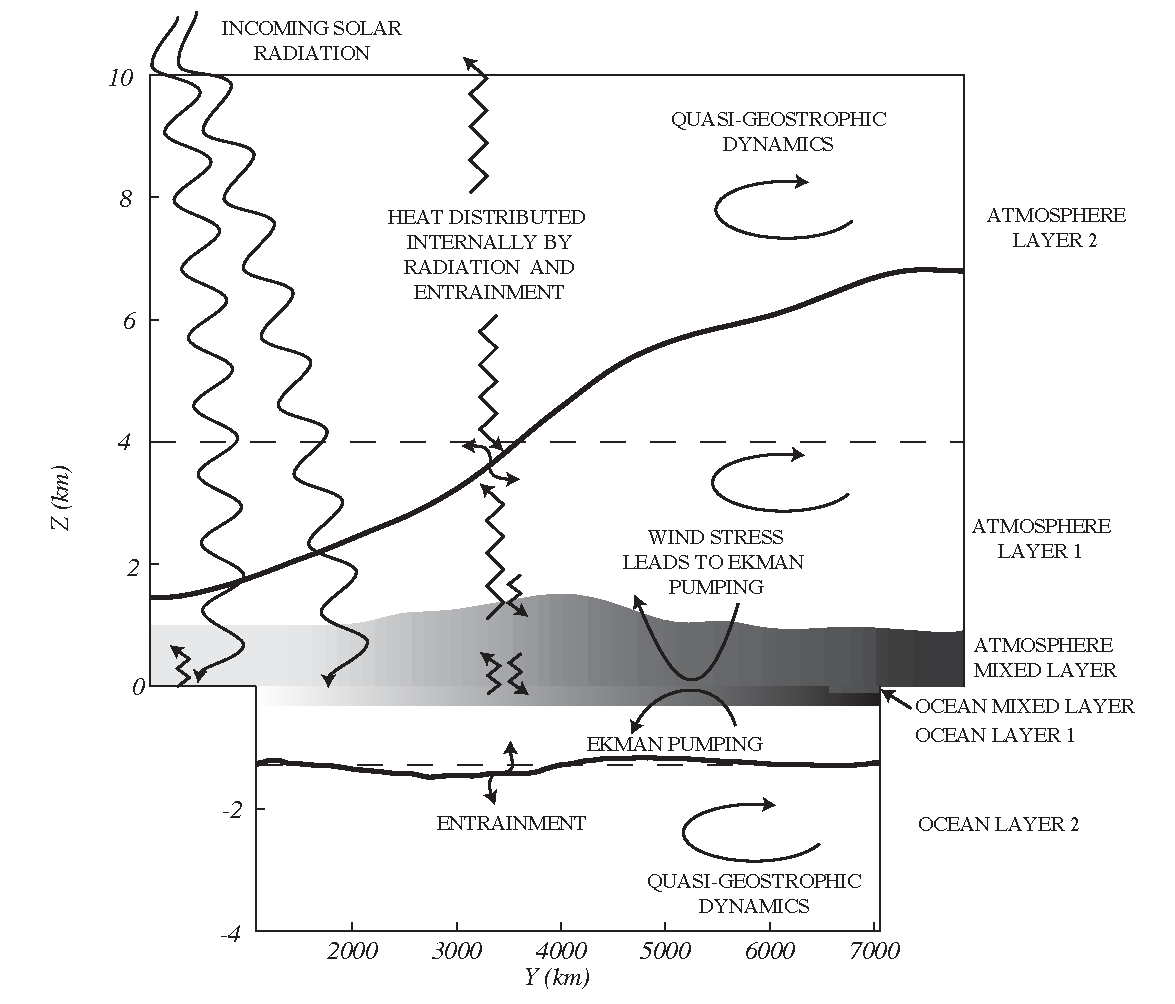
\includegraphics[width=\hsize]{sketch}
\caption{\small Schematic of (a two-layer version of) the Open Quasi-Geostrophic Model. This
meridional slice through the model shows the interface dividing the two QG
dynamical layers in both the ocean and the atmosphere. The mixed layers,
shown by the shading which represents temperature, act to distribute heat
and momentum between the two domains. The model is driven by latitudinally
varying solar forcing, and by redistribution of heat by longwave radiation
in the atmosphere.\label{fig:sketch}}
\end{figure}

This document describes version 1.0.0 of OpenQG.
OpenQG is a fork of version 1.4.0 of the Q-GCM project.
The first version of the Q-GCM code was outlined in \citet{hogg:03b} and \citet{hogg:03c}.
Version 1.2 of Q-GCM was used for systematic ocean-only \citep{hogg:05a} and coupled climate \citep{hogg:06a,hogg:07} studies.
Version 1.3 was used primarily for studies on the variability of the southern ocean climate system \citep{hogg:06c,meredith:06,hogg:08b}.
Version 1.4 was designed to incorporate different wind stress algorithms and has been used to investigate the effects of ocean-atmosphere velocity differences upon stress \citep{hutchinson:10} and, with further modifications, temperature feedback upon oceanic wind stress \citep{hogg:09}.
The current version of OpenQG is designed to port the code from Fortran 77 to Fortran 90 and to introduce an open source development model.

\section{Quasi-Geostrophic equations}\label{sec:qg}
Begin with the equations for conservation of momentum in a rotating fluid,
\begin{equation}\label{eq:mom}
\vc{u}_t + \vc{u}\cdot\nabla\vc{u} - f(\vc{u}\times\vc{\hat{z}}) = -\nabla p -g\vc{\hat{z}} + K\nabla^2\vc{u},
\end{equation}
where we have used $\vc{u}=(u,v,w)$ for velocity, and subscripts to represent partial derivatives.
The pressure $p$ has been rescaled by mean density $\rho$ and we represent viscosity using a constant diffusion coefficient $K$.
The Coriolis parameter has been represented by $f$ and gravitational acceleration by $g$.
The other equations required here are the continuity equation
\begin{equation}\label{eq:cont}
\nabla\cdot\vc{u} = 0,
\end{equation}
and the mass conservation equation which we write as
\begin{equation}\label{eq:temp}
\rho_t + \vc{u}\cdot\nabla\rho = K_H\nabla^2\rho.
\end{equation}

To derive the quasi-geostrophic equations which govern the model dynamics, we simplify (\ref{eq:mom})--(\ref{eq:temp}).
This could be done rigorously by first non-dimensionalising, and then by scaling away less important terms, but it will suffice for now to do this informally.
We begin by assuming, for the purposes of finding the zeroth order equations, that
\begin{enumerate}
\item Vertical velocity is small compared with horizontal velocities;
\item The Coriolis parameter is represented by the frozen $\beta$-plane approximation $f(y)=f_0 + \beta (y - y_0)$ where $f_0$ represents the zeroth order effect of rotation at the central latitude of the domain (i.e. $y = y_0$);
\item Diffusion of momentum is dominated by pressure gradients.
\end{enumerate}
The zeroth order equations in which pressure balances rotation are then
\begin{subequations}
\begin{equation}\label{eq:momxa}
f_0v = p_x,
\end{equation}
\begin{equation}\label{eq:momya}
f_0 u = -p_y,
\end{equation}
\begin{equation}\label{eq:momza}
p_z = - g,
\end{equation}
\end{subequations}
and the continuity equation is
\begin{equation}\label{eq:conta}
u_x + v_y = 0
\end{equation}
which is automatically satisfied by (\ref{eq:momxa}) and (\ref{eq:momya}).
Relative Vorticity is given by
\begin{equation}\label{eq:vort}
\zeta \equiv v_x - u_y = \frac{\nabla_H^2 p}{f_0}.
\end{equation}
The $H$ subscript on the $\nabla$ operator denotes purely horizontal derivatives.

We can now compute the first order quantities (signified by ${}^*$ in the equations below) for the horizontal momentum and continuity equations which include zeroth order horizontal velocity terms and first order pressure and rotation terms,
\begin{subequations}
\begin{equation}\label{eq:momxb}
u_t + uu_x + vu_y  - f_0 v^* - \beta(y-y_0) v = -p_x^* - A_4 \nabla_H^4 u,
\end{equation}
\begin{equation}\label{eq:momyb}
v_t + uv_x + vv_y + f_0 u^* + \beta(y-y_0) u = -p_y^* - A_4 \nabla_H^4 v,
\end{equation}
\end{subequations}
\begin{equation}\label{eq:contb}
\nabla\cdot\vc{u}^* = 0,
\end{equation}
where we have introduced a fourth-order horizontal viscosity scheme (the coefficient $A_4$ is positive for energy dissipation).
First order pressure terms can be eliminated by cross-differentiating (\ref{eq:momxb}) and (\ref{eq:momyb}), giving
\begin{multline}
u_{ty} + (uu_x)_y + (vu_y)_y  - f_0 v^*_y - [\beta(y-y_0) v]_y + A_4\nabla_H^4 u_y\\
= v_{tx} + (uv_x)_x + (vv_y)_x + f_0 u^*_x + [\beta(y-y_0) u]_x + A_4\nabla_H^4 v_x,
\end{multline}
and rearranging:
\begin{multline}
\zeta_t +\left(u\left[\zeta + \beta(y-y_0)\right]\right)_x +\left(v\left[\zeta + \beta(y-y_0)\right]\right)_y + \\
(u_x + v_y)\left[\zeta + \beta(y-y_0)\right] + f_0 (u^*_x + v^*_y)  = - A_4\nabla_H^4\zeta
\end{multline}
Insert (\ref{eq:conta}) and (\ref{eq:contb}) to eliminate zeroth order divergence terms and first order velocities, leaving an equation which depends only upon zeroth order terms
\begin{multline}\label{eq:momxi}
\left[\zeta + \beta(y-y_0)\right]_t +\left(u\left[\zeta + \beta(y-y_0)\right]\right)_x +\left(v\left[\zeta + \beta(y-y_0)\right]\right)_y = f_0 w^*_z - A_4\nabla_H^4 \zeta.
\end{multline}
Relative vorticity is given by
\begin{equation}\label{eq:relvort}
q^* \equiv \zeta + \beta(y - y_0),
\end{equation}
which lets us write (\ref{eq:momxi}) as
\begin{equation}\label{eq:momxi2}
q^*_t +\left(uq^*)\right)_x +\left(vq^*\right)_y = f_0 w^*_z - A_4\nabla_H^4 \zeta.
\end{equation}

\subsection{Layer equations}
We now integrate (\ref{eq:momxi2}) over the layer depth.
In doing this we introduce some new notation.
Layer variables are indexed with subscript $k$ from 1 to $N$, increasing upwards.
Layer interface variables are indexed with subscripts $l$ from 0 to $N$.
For a layer interface variable $X$ we introduce the function
\begin{equation}
\delta(X)_k = X_{l=k} - X_{l=k-1} \quad \quad \textrm{for }k = 1..N.
\end{equation}
Similarly, for a layer variable $Y$ we introduce the function
\begin{equation}
\delta(Y)_l = Y_{k=l+1} - Y_{k=l} \quad \quad \textrm{for }l = 1..N-1.
\end{equation}

Note that it is assumed that $p_k$, $u_k$ and $v_k$ are effectively layer-averaged quantities, so that integration between $H_{l=k-1}$ and $H_{l=k}$ simply gives
\begin{equation}\label{eq:momq}
\left(q^*_k\right)_t  + \left(u_k q^*_k \right)_x  + \left(v_kq^*_k\right)_y  = \frac{f_0 \delta(w^*)_k}{\delta(H)_k} - A_4\nabla_H^4\zeta_k,
\end{equation}
which is an equation for the evolution of potential vorticity in the layer.
\subsection{Vertical velocity}
Evaluation of vertical velocity at the layer boundaries requires knowledge of the flux between layers (which we call $e_l$ for net entrainment velocity through the boundary of the layer).
Vertical velocity is a first order quantity and thus incorporates variable layer interface pertubation height $\eta_l$, giving
\begin{equation}\label{eq:w2}
\delta\left(w^*\right)_k =  \left(\delta(\eta)_k\right)_t + \left(u_k \delta(\eta)_k\right)_x + \left(v_{k} \delta(\eta)_k\right)_y + \delta(e)_k.
\end{equation}
We define the pertubation interface height
\begin{eqnarray}
\eta_{l} & \equiv &  \frac{\delta(p)_l}{\gp{}{l}}\label{eq:eta1}.
\end{eqnarray}
Here we have introduced $\gp{}{l}$, the reduced gravity across the $l^\textrm{th}$ interface, given by
\begin{eqnarray}
\gp{}{l}   & = & \frac{g\delta(\rho)_l}{\rhb{}_0}.
\end{eqnarray}
The value of $\eta$ at the upper and lower boundaries of the domain cannot be expclitly calculated with the above equations, and thus depend on the defined boundary conditions.
At the ocean-atmosphere interface and the top of the atmosphere the pertubation interface height is defined to be zero, so
\begin{equation}
\eta_N = 0.
\end{equation}
At the bottom of both the atmosphere and ocean the pertubation interface height is given by the topography/bathymetry, so
\begin{equation}
\eta_0 = D - H_0,
\end{equation}
where the atmospheric topography is zero over the ocean and is assumed to be small compared with the unperturbed layer thickness $\delta(H)_1$, for consistency with the quasigeostrophic scaling.

Combining (\ref{eq:momq}) and (\ref{eq:w2}) gives
\begin{equation}
\left(q^*_k - \frac{f_0\delta(\eta)_k}{\delta(H)_k}\right)_t  + \left(u_k \left(q^*_k - \frac{f_0\delta(\eta)_k}{\delta(H)_k}\right)\right)_x  + \left(v_k\left(q^*_k -\frac{f_0\delta(\eta)_k}{\delta(H)_k}\right)\right)_y  = \frac{f_0 \delta(e)_k}{\delta(H)_k} - A_4\nabla_H^4\zeta_k.
\end{equation}
We now define the layer potential vorticity as
\begin{equation}\label{eq:layerpv}
q_k \equiv \frac{\nabla_H^2 p_k}{f_0} + \beta(y - y_0) - \frac{f_0\delta(\eta)_k}{\delta(H)_k},
\end{equation}
which lets us write
\begin{equation}\label{eq:dynamic}
\left(q_k\right)_t  + \left(u_kq_k\right)_x  + \left(v_kq_k\right)_y  = \frac{f_0 \delta(e)_k}{\delta(H)_{k}} - A_4\nabla_H^4\zeta_k.
\end{equation}

\subsection{Vector equations}

So far we have written all equations with respect to a particular layer. We now write down the equations in terms of length $N$ vectors. Equation (\ref{eq:dynamic}) can be written
\begin{equation}\label{eq:qt}
\vc{q}_t  + \left(\vc{u}\vc{q}\right)_x  + \left(\vc{v}\vc{q}\right)_y  = \mtx{B}\vc{e} + \frac{A_2}{f_0}\nabla_H^4\vc{p} - \frac{A_4}{f_0}\nabla_H^6\vc{p},
\end{equation}
where an additional laplacian diffusion term is included. The matrix $\mtx{B}$ is
\begin{equation}
\mtx{B} = f_0
\left[ \begin{array}{cccccc}
\frac{-1}{\delta(H)_1} & \frac{1}{\delta(H)_1} & &\\
 & \frac{-1}{\delta(H)_2} & \frac{1}{\delta(H)_2} &\\
 & &  \cdot & \cdot \\
 & &  & \cdot & \cdot \\
 & &   & & \frac{-1}{\delta(H)_N}& \frac{1}{\delta(H)_N} \\
 \end{array}\right].
\end{equation}
Note that $\vc{e}$ is a vector of length $N+1$ which is yet to be determined.
(\ref{eq:qt}) can also be written as
\begin{equation}\label{eq:qt2}
\vc{q}_t  = \frac{1}{f_0} J(\vc{q},\vc{p}) + \mtx{B}\vc{e}  + \frac{\at{}}{f_0}\nabla_H^4 \vc{p} - \frac{\ah{}}{f_0}\nabla_H^6 \vc{p},
\end{equation}
where $J$ is the Jacobian,
\[J(\vc{q},\vc{p}) =\vc{q}_x\vc{p}_y - \vc{q}_y\vc{p}_x.\]
Equation (\ref{eq:layerpv}) can be written
\begin{equation}\label{eq:layerpv2}
\vc{q} = \frac{\nabla_H^2 \vc{p}}{f_0} + \beta(y - y_0) - f_0\left(\mtx{A}\vc{p} + \vc{D}\right),
\end{equation}
where $\mtx{A}$ is an $N\times N$ matrix representing the linear coefficients of pressure in the pertubation interface height equations and $\vc{D}$ is a vector representing the topography/bathymetry boundary conditions. 
We write
\begin{equation}\label{eq:mata}
\mtx{A} =
\left[ \begin{array}{cccccc}
    \frac{-1}{\delta(H)_1 \gp{}{1}} & \frac{1}{\delta(H)_1 \gp{}{1}} &&\\
    \frac{1}{\delta(H)_2 \gp{}{1}}  & \frac{-1}{\delta(H)_2}\left(\frac{1}{\gp{}{1}} + \frac{1}{\gp{}{2}}\right) & \frac{1}{\delta(H)_2 \gp{}{2}} &\\
&  \cdot & \cdot& \cdot\\
 &&  \cdot & \cdot& \cdot\\
&  & &   \frac{1}{\delta(H)_N \gp{}{N-1}}& \frac{-1}{\delta(H)_N \gp{}{N-1}} \\
 \end{array}\right]
\end{equation}
and
\begin{equation}\label{eq:matda}
\Dt{} =
\left[ \begin{array}{c}
\frac{D - H_0}{\delta(H)_1}\\
0\\
\cdot\\
\cdot\\
0\\
 \end{array}\right].
\end{equation}
We can write (\ref{eq:layerpv2}) in operator form as
\begin{equation}\label{eq:layerpv3}
\left(\nabla_H - f^2_0\mtx{A} \right)\vc{p}  = f_0\left(\vc{q} - \beta(y - y_0) - f_0\vc{D}\right).
\end{equation}
Given appropriate intial and boundary conditions, equations (\ref{eq:qt2}) and (\ref{eq:layerpv2}) allow us to solve for layer potential vorticity $\vc{q}$ and layer pressure $\vc{p}$ forced by entrainment $\vc{e}$.

\subsection{Boundary conditions}
The boundary conditions in the model are applied to the pressure field.
In the case of the finite box ocean the boundary pressure is given by
\begin{equation}\label{eq:bc1}
\p{o}{k} = \f{o}{k}(t),
\end{equation}
where the function $\f{o}{k}(t)$ is determined by constraints on mass
(see section \ref{app:boxcon}), and is constant around the boundary. 
For the atmosphere, or the cyclic ocean case, the east and west
boundaries are periodic, and pressure on the north and south boundaries
satisfies a more complicated mixed condition derived using
both mass and momentum constraints, after \citet{mcwilliams:77}
(see sections \ref{app:discon} and \ref{app:chancon}). 
The values on the north and south boundaries will differ. 
As these are mixed conditions rather than simply specified values of pressure, they do not amount to a simple flux condition.

Boundary conditions are also required for the derivatives of pressure on all solid boundaries, and in all cases we use another form of mixed condition, applied to the normal derivatives, following \citet{haidvogel:92}.
For the north and south boundaries of the atmosphere, these are written as
\begin{equation}\label{eq:bc2}
\p{a}{k}_{nn} = -  \frac{\alphbc{a}}{\Delta} \p{a}{k}_n,
\end{equation}
\begin{equation}\label{eq:bc3}
\p{a}{k}_{4n} = - \frac{\alphbc{a}}{\Delta} \p{a}{k}_{3n},
\end{equation}
where the nondimensional coefficient $\alphbc{}$ is zero for free slip and infinite for no-slip boundary conditions (although, in practice, $\alphbc{}>2$ is a good approximation to no-slip), $\Delta$ is the horizontal grid spacing and subscript $n$ denotes the outward normal derivative.
Again, the east and west boundaries are periodic. 
The cyclic ocean case is handled in the same way as the atmosphere. For the finite box ocean, (\ref{eq:bc2}) and (\ref{eq:bc3}) are also applied to the west and east boundaries.

\subsection{Ekman layer drag}
It is relevant at this stage to note that momentum must be lost from the ocean, and that this occurs via drag due to a no-slip condition at the ocean floor.
We calculate this by assuming an Ekman layer of prescribed thickness  $\delek= \sqrt{K/\lvert f_0\rvert}$ and calculate the Ekman pumping when a stress term is included.
In this case there is no need to calculate stress explicitly, and so we determine the Ekman pumping directly from pressure.
Velocity in the Ekman layer will be given by
\begin{subequations}
\begin{equation}
\vv{}{1} = \frac{\p{}{1}_x}{f_0} + \frac{\tx{}{x}}{\delek f_0},
\end{equation}
\begin{equation}
\uu{}{1} = -\frac{\p{}{1}_y}{f_0} - \frac{\tx{}{y}}{\delek f_0}.
\end{equation}
\end{subequations}
We use linear stress,
\begin{equation}
(\tx{}{x},\tx{}{y}) = \frac{K}{\delek}(\uu{}{1},\vv{}{1}),
\end{equation}
so that
\begin{subequations}
\begin{equation}
\vv{}{1} = \frac{\p{}{1}_x}{f_0} + \textrm{sgn}(f_0) \uu{}{1},
\end{equation}
\begin{equation}
\uu{}{1} = -\frac{\p{}{1}_y}{f_0} -  \textrm{sgn}(f_0) \vv{}{1}.
\end{equation}
\end{subequations}
Combining these two we can write separate equations for each component of velocity,
\begin{subequations}
\begin{equation}
\vv{}{1} = \frac{\p{}{1}_x}{2f_0} -\frac{\p{}{1}_y}{2 \lvert f_0 \rvert},
\end{equation}
\begin{equation}
\uu{}{1} = -\frac{\p{}{1}_y}{2f_0} - \frac{\p{}{1}_x}{2 \lvert f_0 \rvert }.
\end{equation}
\end{subequations}
These can be substituted into (\ref{eq:cont}), which is then integrated across the Ekman layer:
\begin{equation}\label{eq:contz}
\ww{}{0} = \frac{\delek}{2 \lvert f_0 \rvert } \nabla_H^2\p{}{1}.
\end{equation}
This vertical velocity on the lower boundary of the ocean alters the vertical velocity in ocean layer $1$ but has no impact on the heat flux (as there is no temperature gradient).


\section{Mixed layers}\label{sec:mixed}
Quasi-geostrophy describes, to first order, the dynamics of both ocean and atmosphere, but cannot handle the fluxes of heat and momentum between these two domains which are required for a coupled model.
OpenQG addresses this difficulty by embedding mixed layers within the interface layer of both ocean and atmosphere.
In its current form the mixed layers do not include parameterisation of humidity in the atmosphere or salinity in the ocean, and therefore exchanges of these quantities are not modelled.
Nonetheless, the most fundamental processes -- transfer of momentum from atmosphere to ocean, and flux of heat in both directions -- are included.

\subsection{Mixed layer stress}\label{sec:mix1}
We first derive the stress at the ocean-atmosphere interface by finding the atmospheric mixed layer velocities.
The distinction between mixed layer and layer 1 velocities is that the mixed layer is thin enough that the vertical flux of horizontal momentum is significant.
The zeroth order momentum equations can be found by including the vertical flux of momentum by a dynamic stress (rescaled by mean density $\rhb{a}$)
\begin{subequations}
\begin{equation}
- f_0 \vv{a}{m} = -\p{a}{1}_x + \tx{a}{x}_z,
\end{equation}
\begin{equation}
 f_0 \uu{a}{m} = -\p{a}{1}_y + \tx{a}{y}_z.
\end{equation}
\end{subequations}
Assuming a fixed atmospheric mixed layer thickness and zero stress at the upper boundary of the mixed layer, we substitute (\ref{eq:momxa},b) and integrate over mixed layer depth $\HH{a}{m}$ to give
\begin{subequations}
\begin{equation}\label{eq:vtau}
\vv{a}{m} = \vv{a}{1} + \frac{\tx{a}{x}}{\HH{a}{m}f_0},
\end{equation}
\begin{equation}\label{eq:utau}
\uu{a}{m} = \uu{a}{1} - \frac{\tx{a}{y}}{\HH{a}{m}f_0},
\end{equation}
\end{subequations}
where it is implied that stress is a layer-averaged quantity.
Following the results of \citet{duhaut:06} demonstrating the sensitivity of ocean energetics to wind stress written as the difference between atmospheric and ocean mixed layer velocities, we now write the stress as
\begin{equation}\label{eq:stress2}
(\tx{a}{x},\tx{a}{y}) = C_D \lvert \vc{\uu{a}{m}} - \vc{\uu{o}{m}} \rvert (\uu{a}{m} - \uu{o}{m},\vv{a}{m} - \vv{o}{m}),
\end{equation}
$C_D$ being a dimensionless drag coefficient.
Here we also need to know that 
\begin{subequations}
\begin{equation}\label{eq:vtauoc}
\vv{o}{m} = \vv{o}{N} - \frac{\tx{o}{x}}{\HH{o}{m}f_0},
\end{equation}
\begin{equation}\label{eq:utauoc}
\uu{o}{m} = \uu{o}{N} + \frac{\tx{o}{y}}{\HH{o}{m}f_0},
\end{equation}
\end{subequations}
(note the change in sign from \ref{eq:vtau}, \ref{eq:utau}).
Atmospheric and oceanic dynamic stress are related by the density ratio,
\begin{equation}\label{eq:ocstr2}
\tx{o}{} =  \frac{\rhb{a}}{\rhb{o}}\tx{a}{}.
\end{equation}

For simplicity, we define the following parameters 
\[M \equiv \lvert \vc{\uu{a}{m}} - \vc{\uu{o}{m}} \rvert \ge 0\]
\[a \equiv \frac{C_D}{\HH{a}{m}f_0}\]
\[b \equiv \frac{\rhb{a}C_D}{\rhb{o}\HH{o}{m}f_0} \approx 10^{-2}a\]
We can then write
\begin{equation}\label{eq:stress3}
(\tx{a}{x},\tx{a}{y}) = C_D M (\uu{a}{m} - \uu{o}{m},\vv{a}{m} - \vv{o}{m}).
\end{equation}

Substituting (\ref{eq:stress3}) into (\ref{eq:vtau},b) gives
\begin{subequations}
\begin{equation}
\vv{a}{m} = \vv{a}{1} + a M (\uu{a}{m} - \uu{o}{m}),
\end{equation}
\begin{equation}
\uu{a}{m} = \uu{a}{1} - a M (\vv{a}{m} - \vv{o}{m}).
\end{equation}
\end{subequations}
We also substitute (\ref{eq:stress3}) into (\ref{eq:vtauoc},b) giving
\begin{subequations}
\begin{equation}
\vv{o}{m} = \vv{o}{N} - b M (\uu{a}{m} - \uu{o}{m}),
\end{equation}
\begin{equation}
\uu{o}{m} = \uu{o}{N} + b M (\vv{a}{m} - \vv{o}{m}).
\end{equation}
\end{subequations}
The ocean equations above can be subtracted from the atmosphere equations to give
\begin{subequations}
\begin{equation}\label{eq:veldif1}
(\vv{a}{m} - \vv{o}{m}) =  (\vv{a}{1} - \vv{o}{N}) + (a + b) M (\uu{a}{m} - \uu{o}{m}),
\end{equation}
\begin{equation}\label{eq:veldif2}
(\uu{a}{m} - \uu{o}{m}) = (\uu{a}{1} - \uu{o}{N}) - (a + b) M (\vv{a}{m} - \vv{o}{m}),
\end{equation}
\end{subequations}
which can be rewritten as 
\begin{subequations}
\begin{equation}\label{eq:veldif1a}
(\vv{a}{m} - \vv{o}{m}) -  (a + b) M (\uu{a}{m} - \uu{o}{m}) =  (\vv{a}{1} - \vv{o}{N}) ,
\end{equation}
\begin{equation}\label{eq:veldif2a}
(\uu{a}{m} - \uu{o}{m}) + (a + b) M (\vv{a}{m} - \vv{o}{m})= (\uu{a}{1} - \uu{o}{N}).
\end{equation}
\end{subequations}
We square these equations,
\begin{subequations}
\begin{equation}
(\vv{a}{m} - \vv{o}{m})^2 - 2 (a + b) M (\uu{a}{m} - \uu{o}{m})(\vv{a}{m} - \vv{o}{m}) + (a+b)^2 M^2(\uu{a}{m} - \uu{o}{m})^2 =  (\vv{a}{1} - \vv{o}{N}) ^2,
\end{equation}
\begin{equation}
(\uu{a}{m} - \uu{o}{m})^2 + 2 (a + b) M (\uu{a}{m} - \uu{o}{m}) (\vv{a}{m} - \vv{o}{m}) + (a + b)^2 M^2 (\vv{a}{m} - \vv{o}{m})^2= (\uu{a}{1} - \uu{o}{N})^2,
\end{equation}
\end{subequations}
and add to give
\begin{equation}
M ^2 + (a+b)^2 M^4 =  \lvert \vc{\uu{a}{1}} - \vc{\uu{o}{N}} \rvert ^2.
\end{equation}
Since layer 1 velocities are already known, we can now solve the quadratic equation to give 
\begin{equation}
M = \frac{1 }{\sqrt{2}\, \lvert a+b \rvert} \sqrt{-1 +\sqrt{1 + 4 (a+b)^2 \lvert \vc{\uu{a}{1}} - \vc{\uu{o}{N}} \rvert ^2}}.
\end{equation}
We choose the positive root of the quadratic because that is the solution which $\to 0$ as $|\uu{a}{1}-\uu{o}{N}| \to 0$ as is required.

Stress can then be calculated from cross-substitution of (\ref{eq:veldif1a}) and (\ref{eq:veldif2a})
\begin{subequations}
\begin{align}
(\vv{a}{m} - \vv{o}{m}) (1 +  (a + b)^2 M^2) =  (\vv{a}{1} - \vv{o}{N}) + (a + b) M (\uu{a}{1} - \uu{o}{N}) ,\label{eq:veldif3}\\
(\uu{a}{m} - \uu{o}{m})(1 +  (a + b)^2 M^2) = (\uu{a}{1} - \uu{o}{N}) - (a + b) M  (\vv{a}{1} - \vv{o}{N}) ,
\end{align}
\end{subequations}
which, in combination with (\ref{eq:stress2}) gives
\begin{subequations}
\begin{equation}\label{eq:stress4}
\tx{a}{x}  =  C_D M \frac{(\vv{a}{1} - \vv{o}{N}) + (a + b) M (\uu{a}{1} - \uu{o}{N}) }{1 +  (a + b)^2 M^2},
\end{equation}
\begin{equation}\label{eq:veldif4}
\tx{a}{y} =  C_D M \frac{(\uu{a}{1} - \uu{o}{N}) - (a + b) M  (\vv{a}{1} - \vv{o}{N})} {1 +  (a + b)^2 M^2},
\end{equation}
\end{subequations}

A second distinction between mixed layer and interface layer velocities exists because the ageostrophic mixed layer velocities have a divergent component which produces vertical Ekman velocities.
Ekman pumping is calculated using the continuity equation (\ref{eq:cont}) integrated from $0$ to $\HH{a}{m}$,
\begin{equation}\label{eq:wek1}
 \ek{a} = - \HH{a}{m} \uu{a}{m}_x - \HH{a}{m} \vv{a}{m}_y,
\end{equation}
where we use $\ww{a}{m}(0)=0$ and $\ww{a}{m}(\HH{a}{m}) = \ek{a}$.
Substitute velocity from (\ref{eq:vtau},b), giving
\begin{equation}\label{eq:atek}
\ek{a}  = \frac{\tx{a}{y}_x - \tx{a}{x}_y}{f_0},
\end{equation}
the familiar expression for Ekman velocity as a function of stress.

The ocean mixed layer is essentially an inversion of the atmospheric mixed layer.
The difference here is that stress in the oceanic mixed layer is passive,  depending entirely on wind stress and the atmosphere to ocean density ratio as per (\ref{eq:ocstr2}).
$\tx{o}{}$ is now computed at ocean resolution directly from the velocity shear,
and Ekman pumping in the ocean surface layer is obtained in a similar fashion to $\ek{a}$:
\begin{equation}\label{eq:ocek}
\ek{o}  = \frac{\tx{o}{y}_x - \tx{o}{x}_y}{f_0}.
\end{equation}


\subsection{Mixed layer evolution}
The mixed layers also act to transfer heat between atmosphere and ocean.
To allow this, we need to explicitly calculate the evolution of temperature in the mixed layers.
As before we integrate over the mixed layer thickness,  but for the purposes of temperature evolution we allow perturbations $\etb{a}{m} = \h{a}{m} - \HH{a}{m} $ to mixed layer thickness in the atmosphere only.
The variable mixed layer thickness is needed in the atmosphere because of an observed instability which occurs due to large vertical heat transports in regions where there is a coherent pattern of upwelling and cold mixed layer temperatures.

To find the evolution of mixed layer thickness, we again integrate the continuity equation, this time from $0$ to $\h{a}{m}$,
\begin{equation}\ww{a}{m}(\h{a}{m}) = - \h{a}{m}\uu{a}{mx} - \h{a}{m}\vv{a}{my}.\end{equation}
Now we write an equation for the mixed layer thickness, analogous to (\ref{eq:w2}),
\begin{equation}\label{eq:w0a}
\ww{a}{m}(\h{a}{m}) = \h{a}{m}_t + \uu{a}{m}\h{a}{mx} + \vv{a}{m} \h{a}{my}  + \e{a}{m}.
\end{equation}
Combining these gives the evolution equation for mixed layer thickness, which implicitly includes the Ekman divergence terms,
\begin{equation}\label{eq:hevmat}
\h{a}{m}_t + (\uu{a}{m}\h{a}{m})_x + (\vv{a}{m} \h{a}{m})_y =   - \e{a}{m}.
\end{equation}
This equation is solved with $\h{a}{m} = \HH{a}{m}$ on the north and south boundaries.

The evolution of mixed layer temperature comes from a heat equation,
\begin{equation}\label{eq:tempa}
\T{a}{mt} + \uu{a}{m} \T{a}{mx} + \vv{a}{m} \T{a}{my} + \ww{a}{m} \T{a}{mz} =  \kh{a} \nabla_H^2 \T{a}{m} - \kf{a}\nabla_H^4\T{a}{m} - \frac{{}^aF_z}{\rhb{a} \cp{a}},
\end{equation}
where $\cp{a}$ is the specific heat capacity and $\kh{a}$ a diffusion coefficient.
This equation includes a fourth-order diffusion term with positive coefficient $\kf{a}$ for numerical stability.
We have chosen to retain the horizontal diffusion terms, while writing the vertical diffusion as the vertical gradient of a flux ${}^aF$ of heat energy.
Note that flux is defined positive upwards so that a positive flux gradient will act to cool the layer in a stably stratified fluid.
Integrate (\ref{eq:tempa}) between $0$ and $\h{a}{m}$, \begin{equation}\label{eq:tempc}
\T{a}{mt} + (\uu{a}{m} \T{a}{m})_x + (\vv{a}{m} \T{a}{m})_y + \frac{\ek{a}\T{a}{m}}{\HH{a}{m}}  =  \kh{a} \nabla_H^2 \T{a}{m} - \kf{a}\nabla_H^4\T{a}{m}+ \frac{-\F{a}{m}{} + \F{a}{0}{}}{\rhb{a} \cp{a} \h{a}{m}}.
\end{equation}
The fluxes at the top of the mixed layer ($\F{a}{m}{}$) and at the surface ($\F{a}{0}{}$) are derived in \S \ref{sec:flux} below.
There is no heat flux on the north and south boundaries.

In the ocean, we use a constant thickness mixed layer, and the equivalent equation to (\ref{eq:tempc}) is
\begin{equation}\label{eq:tempd}
\T{o}{mt} + (\uu{o}{m} \T{o}{m})_x + (\vv{o}{m}  \T{o}{m})_y - \frac{\ek{o}\T{o}{m}}{\HH{o}{m}}  =  \kh{o}  \nabla_H^2 \T{o}{m}  - \kf{o}  \nabla_H^4 \T{o}{m}   + \frac{- \F{o}{0}{} + \F{o}{m}{}}{\rhb{o} \cp{o} \HH{o}{m}}.
\end{equation}
The default boundary conditions for the ocean mixed layer evolution are zero heat flux.
However, provision is made for constant temperature boundary conditions on the equatorward meridional boundary, the value of the temperature there being determined from radiative balance.
This condition is necessary because advection and diffusion of warm tropical water from that boundary are not explicitly included in the model.
A similar boundary condition is not required on the poleward meridional boundary because convection is active there.


\section{Heat flux between layers}\label{sec:flux}
OpenQG includes flux of heat between each layer due to a number of different processes.
We derive each case below, and write heat flux as the superposition of a mean and a first order perturbation quantity, so that fluxes are linearised about a mean state in which the model is in radiative balance.

\subsection{Incoming solar flux}
The incoming solar radiation is written as a heat flux $F_s$.
The atmosphere is transparent to incoming shortwave radiation which is deposited directly in the oceanic mixed layer.
Over land, incoming shortwave is absorbed by the land and immediately re-emitted as longwave radiation into the atmospheric mixed layer.
Heat flux is defined so that positive fluxes denote an upwards movement of heat energy, so that the mean incoming radiation, $\overline{F_s}$, is defined negative.
We thus divide the radiation into a mean and a $y$-dependent part which integrates to zero over the domain,
\begin{equation}\label{eq:fspy}
F_s(y) =  \overline{F_s} + \frac{F_s'}{2} \sin\left( \frac{\pi (y - y_0)}{{}^aY}\right),
\end{equation}
where ${}^aY$ is the latitudinal atmospheric domain size.
The magnitude of $F_s'$ is defined in \verb=input.params=, and it has the same sign as $f_0$ (i.e. positive for the northern hemisphere and negative for the southern hemisphere).

\subsection{Radiative fluxes} \label{sub:rad}
Each atmospheric layer, and the oceanic mixed layer, radiates and absorbs heat depending upon its temperature and optical depth.
The emitted longwave radiation is either absorbed, transmitted or partially transmitted by neighbouring layers.
The equations describing radiative flux from each layer are given below, in the form of a mean part plus linear perturbations.
The constant coefficients governing the linear response of the model are derived in appendix \ref{app:rad}.

\begin{description}
\item[Oceanic Mixed Layer] absorbs all downgoing longwave radiation (as well as incoming shortwave radiation) which passes through the atmospheric mixed layer.
Emits radiation according to
\begin{equation}
\Fup{0} \approx \overline{\Fup{0}} + \dup{0}\T{o}{m}'.
\end{equation}

\item[Atmospheric Mixed Layer] absorbs all downgoing and upgoing longwave radiation.
Linearised radiation is written
\begin{equation}\label{eq:fmup}
\Fup{m} \approx \overline{\Fup{m}} + \bup{m} \etb{a}{m} + \cupp{m} \D{a} + \dup{m} \T{a}{m}',
\end{equation}
\begin{equation}\label{eq:fmdown}
\Fdown{m} \approx \overline{\Fdown{m}} + \ddown{m}\T{a}{m}' .
\end{equation}

\item[Atmospheric QG layers] have a more complicated radiation balance, as partial absorption of incoming radiation and partial emission of the incoming radiation occur:
\begin{equation}\label{eq:fkup}
\Fup{k} \approx \overline{\Fup{k}} + \sum_{i=1}^{\textrm{min}(k,N-1)}\aup{k,i}\etb{a}{i} + \bup{k} \etb{a}{m} + \cupp{k} \D{a} + \dup{k}\T{a}{m}'\quad \quad \textrm{for }k=1,N,
\end{equation}
\begin{equation}\label{eq:fkdown}
\Fdown{k} \approx \overline{\Fdown{k}} + \sum_{i=\max(k-1,1)}^{N-1} \adown{k,i} \etb{a}{i} + \bdown{k} \etb{a}{m} + \cdown{k} \D{a} \quad \quad \textrm{for }k=1,N.
\end{equation}
\end{description}

\subsection{Sensible and latent heat flux}
Sensible and latent heat flux from the oceanic to the atmospheric mixed layer is represented by
\begin{equation}
F_{\lambda}=\lambda(\T{o}{m} - \T{a}{m}),
\end{equation}
or in perturbation form
\begin{equation}
F_{\lambda}=\overline{F_{\lambda}} + \lambda(\T{o}{m}' - \T{a}{m}'),
\end{equation}
where
\begin{equation}
\overline{F_{\lambda}}=\lambda(\overline{\T{o}{m}} - \overline{\T{a}{m}}).
\end{equation}

\subsection{Entrainment heat flux}
The QG layers have constant (but different) potential temperatures.
Therefore, the combined heat content of any two layers can only change when the interface dividing the layers changes its height.
The entrainment $\e{a}{k}$ therefore implies a vertical heat flux between layers $k$ and $k+1$.
This heat flux is written as a double-sided flux \citep[see][]{mcdougall:98}, so that in the atmosphere
\begin{equation}\label{eq:fent2}
\F{a}{k}{e+} - \F{a}{k}{e-} = - \rhb{a} \cp{a} \e{a}{k} \dt{a}{k},
\end{equation}
where $\dt{a}{k}$ is the change in temperature across the interface and $\F{a}{k}{e+}$ ($\F{a}{k}{e-}$) is the heat flux on the upper (lower) side of interface $k$.
This allows a divergence of heat flux at the interface, but not within the layers.

In the atmosphere we assume no entrainment at the top of the domain:
\begin{equation}
\F{a}{N}{e-} = 0.
\end{equation}
The heat conservation equation in any layer is
\begin{equation}
\F{a}{k}{e-} + \Fup{k} +\Fdown{k+1} = \F{a}{k-1}{e+} + \Fup{k-1}+  \Fdown{k} ,
\end{equation}
allowing calculation of entrainment at the interface $k$ by combining the equations for layers $k$ and $k+1$;
\begin{equation}\label{eq:ent1}
\e{a}{k}  = \frac{\F{a}{k-1}{e+} + \Fup{k-1}+ \Fdown{k}  - \F{a}{k+1}{e-} -\Fup{k+1}  - \Fdown{k+2} }{\rhb{a} \cp{a} \dt{a}{k} }.
\end{equation}
In the 2 layer case this equation is conclusive, since $\F{a}{m}{e+}=0$ (see below) and $\F{a}{N}{e-}=0$ (because it is at the top of the atmosphere), so that we can write the equation for $\e{a}{1}$ explicitly.
For more layers we have insufficient constraints to determine entrainment everywhere.
Therefore, on the basis that most convection and vertical heat transport occurs in the lower atmosphere, we assume that all entrainment occurs at the lowest interface, or in other words
\begin{equation}\label{eq:ent2}
\e{a}{1}  = \frac{\Fup{m}+ \Fdown{1}   -\Fup{N}   }{\rhb{a} \cp{a} \dt{a}{1} }.
\end{equation}
\begin{equation}\label{eq:ent3}
\e{a}{k}  = 0, \quad\quad \textrm{for } k > 1.
\end{equation}
The additional assumption (\ref{eq:ent3}) implies (from \ref{eq:fent2}) that the
interfacial temperature differences $\dt{a}{k}$ are irrelevant for $k > 1$, and thus that the atmospheric layer temperatures $\T{a}{k}$ for $k > 2$ have no thermodynamic significance. 
Their only role then lies in determining the linear response coefficients
in the radiative model (see equations \ref{eq:fluxn} to \ref{eq:adownki}).
All radiation in the atmosphere is therefore encapsulated in (\ref{eq:ent2}), which we now rewrite explicitly in terms of the radiation parameters used in (\ref{eq:fmup}), (\ref{eq:fkup}) and (\ref{eq:fkdown}):
\begin{multline}\label{eq:ent4}
\e{a}{1}  = \frac{1}{\rhb{a} \cp{a} \dt{a}{1} }\biggl[\sum_{k=1}^{N-1}\left(\adown{1,k} - \aup{N,k}\right) \etb{a}{1} + \left(\bup{m} + \bdown{1} - \bup{N} \right) \etb{a}{m} +\\
 \left( \cupp{m} + \cdown{1}  - \cupp{N} \right) \D{a} + \left(\dup{m} - \dup{N}\right) \T{a}{m}'  \biggr] .
\end{multline}

At the mixed layer interface we assume that entrainment is maintained by turbulence on either side of the interface.
In other words, assume
\begin{equation} \F{a}{m}{e+} = \overline{F_x} - \frac{ \rhb{a} \cp{a} \mb{a}{1}}{\HH{a}{1} - \h{a}{m}},\end{equation}
\begin{equation} \F{a}{m}{e-} = \overline{F_x} - \frac{ \rhb{a} \cp{a} \mb{a}{m}}{\h{a}{m}},\end{equation}
where $\overline{F_x}$ is an export heat flux (a constant added heat flux), and
\begin{equation}\frac{ \mb{a}{1}}{\HH{a}{1}-\HH{a}{m}} = \frac{ \mb{a}{m}}{\HH{a}{m}}.\end{equation}
We linearise the above equations to give
\begin{equation} \F{a}{m}{e+} = \overline{F_x} - \frac{ \rhb{a} \cp{a} \mb{a}{1}}{\HH{a}{1} - \HH{a}{m}},\end{equation}
\begin{equation} \F{a}{m}{e-} = \overline{\F{a}{m}{e-}}  - \frac{\rhb{a} \cp{a} \mb{a}{m}}{\HH{a}{m}} \left(1 - \frac{\etb{a}{m}}{\HH{a}{m}}\right).\end{equation}
Then
\begin{equation}\e{a}{m} \approx \frac{\lb{a}{m}}{\rhb{a} \cp{a}\dt{a}{m}} \etb{a}{m},\end{equation}
where
\begin{equation}\lb{a}{m} \equiv \frac{\rhb{a} \cp{a} \mb{a}{m}}{\HH{a}{m} ^2}.\end{equation}
In the model we then use the perturbation forcing
\begin{equation}\F{a}{m}{e-} = \overline{\F{a}{m}{e-}} +  \lb{a}{m} \etb{a}{m}\end{equation}
\begin{equation}\F{a}{m}{e+} =  \overline{\F{a}{m}{e-}} .\end{equation}

In the ocean we assume that the deep layers do not exchange heat so that
\begin{equation}
\F{o}{1}{e-} = 0,
\end{equation}
and heat flux between other layers is zero,
\begin{equation}\label{eq:eok1}
\e{o}{k} = 0, \quad \quad \textrm{for } k > 1.
\end{equation}
Again, the additional assumption (\ref{eq:eok1}) implies that the interfacial temperature differences $\dt{o}{k}$ are irrelevant for $k > 1$, as therefore are the oceanic layer temperatures $\T{o}{k}$ for $k > 2$.
From (\ref{eq:fent2}) we write
\begin{equation}\label{eq:fo1ep}
\F{o}{1}{e+} = - \rhb{o} \cp{o}\e{o}{1}\dt{o}{1}.
\end{equation}
In the oceanic mixed layer, where there is no variation in mixed layer depth, entrainment is solely driven by Ekman pumping,
\begin{equation}
\e{o}{m} = \ek{o}.
\end{equation}
Using a centred difference model for entrainment there, we find
\begin{equation}
\F{o}{m}{e+} = -0.5 \rhb{o} \cp{o}\dt{o}{m} \ek{o},
\end{equation}
\begin{equation}
\F{o}{m}{e-} = 0.5 \rhb{o} \cp{o}\dt{o}{m} \ek{o}.
\end{equation}
Therefore from (\ref{eq:fo1ep}) we can write
\begin{equation}\label{eq:fentp}
\e{o}{1} = - \frac{\dt{o}{m}}{2 \dt{o}{1}} \ek{o}.
\end{equation}
A constant offset is added to $\e{o}{1}$ to ensure its area integral is zero (see appendix \ref{app:occon}).

\section{Layer equations}\label{sec:layers}
We are now in a position to put together equations for each layer.
A schematic of the model which includes radiative fluxes, entrainment velocities and momentum coupling is shown in figure \ref{fig:sketch}.

\subsection{Entrainment}\label{sub:qglayers}
The entrainment vectors are given by
\begin{equation}
\vc{{}^oe} =
\left[ \begin{array}{c}
\ek{o}\\
- \frac{\dt{o}{m}}{2 \dt{o}{1}} \ek{o}\\
0\\
\cdot\\
\cdot\\
\frac{\delek}{2 \lvert f_0 \rvert }\nabla_H^2\p{o}{N}\\
 \end{array}\right]
\end{equation}
and
\begin{equation}\label{eq:ent1a}
\vc{{}^ae} =
\left[ \begin{array}{c}
\ek{a}\\
\frac{\Fup{m}+ \Fdown{1}   - \Fup{N}  }{\rhb{a} \cp{a} \dt{a}{1} }\\
0\\
\cdot\\
\cdot\\
0\\
 \end{array}\right].
\end{equation}
The entrainment equations will be altered if convection occurs.

\subsection{Ocean mixed layer}
From (\ref{eq:tempd}),
\begin{equation}\label{eq:tempda}
\T{o}{mt} + (\uu{o}{m} \T{o}{m})_x + (\vv{o}{m} \T{o}{m})_y  - \frac{\ek{o} \T{o}{m}}{\HH{o}{m}} =  \kh{o}  \nabla_H^2\T{o}{m} - \kf{o}  \nabla_H^4 \T{o}{m}  + \frac{\F{o}{0}{} +  \F{o}{m}{e+}}{\rhb{o} \cp{o}\HH{o}{m} },
\end{equation}
where total oceanic mixed layer forcing is given by
\begin{equation}
\F{o}{0}{} = - F_{\lambda} - \Fup{0} - \Fdown{m} - F_s,
\end{equation}
and we have retained the entrainment flux as a separate term in (\ref{eq:tempda}).
Note that the advective terms here use the mixed layer velocity which is modified by stress, rather than the geostrophic velocity used in (\ref{eq:qt}).

\subsection{Atmosphere mixed layer}
From (\ref{eq:hevmat})  we get
\begin{equation}\label{eq:hevmata}
\h{a}{m}_t + (\uu{a}{m}\h{a}{m})_x + (\vv{a}{m} \h{a}{m})_y =   -\e{a}{m}.
\end{equation}
Note that $\h{a}{m}$ is constrained to prevent very small values occurring: when $\h{a}{m}$ becomes smaller than a critical value, it is reset to the critical value, and $\T{a}{m}$ adjusted accordingly to conserve heat.
Equation (\ref{eq:temp}) gives
\begin{equation}\label{eq:tempca}
\T{a}{mt} + (\uu{a}{m} \T{a}{m})_x + (\vv{a}{m} \T{a}{m})_y + \frac{\ek{a} \T{a}{m}}{\HH{a}{m}}  =  \kh{a} \nabla_H^2 \T{a}{m} - \kf{a}\nabla_H^4\T{a}{m} +\frac{-\F{a}{m}{} + \F{a}{0}{}}{\rhb{a} \cp{a} \h{a}{m}},
\end{equation}
where atmospheric  mixed layer forcing above and below the mixed layer are respectively given by
\begin{equation}\F{a}{m}{} = \Fup{m} + \Fdown{1} + \F{a}{m}{e-}\end{equation}
\begin{equation}\F{a}{0}{} = \begin{cases} \Fdown{m} + F_{\lambda} + \Fup{0} & \text{over ocean,}\\
-F_s' & \text{over land.}
\end{cases}\end{equation}

\subsection{Convection}
Convection will occur when unstable stratification forms and will act to change temperature in the mixed layers in a way which conserves heat.
In the atmosphere, when $\T{a}{m}$ exceeds $\T{a}{1}$ we adjust the layer 1 entrainment as follows,
\begin{equation}\label{eq:atconv}
 \delta \e{a}{1}= \frac{\h{a}{m}(\T{a}{1} - \T{a}{m} )}{2 \Delta^at \dt{a}{1} },
\end{equation}
and set $\T{a}{m} = \T{a}{1}$.
Here we use $\Delta^at$ to represent the atmosphere timestep.

Likewise, in the ocean, when $\T{o}{m} < \T{o}{1}$ we alter layer 1 entrainment by
\begin{equation}\label{eq:occonv}
\delta \e{o}{1}= \frac{ - \HH{o}{m}(\T{o}{1} - \T{o}{m} )}{2 \Delta^ot \dt{o}{1}},
\end{equation}
and set  $\T{o}{m} = \T{o}{1}$.

\section{Mean state}\label{sec:mean}
The mean state is defined by the solution of the above equations when $F_s = \overline{F_s}$.
In this state there will be no motion, so that pressure gradients, vorticity gradients and entrainment disappear.
Our full equation set then reduces to a radiation balance between the atmosphere and the oceanic mixed layer.
From (\ref{eq:ent1a}) we get a heat balance in the upper atmosphere
\begin{equation}\label{eq:ent1b}
\overline{\F{a}{m}{e+}} + \overline{\Fdown{1}} + \overline{\Fup{m}} - \overline{\Fup{N}}=0,
\end{equation}
(\ref{eq:tempca}) gives us the heat balance in the atmospheric mixed layer
\begin{equation}\label{eq:tempcb}
-  \overline{\Fup{m}} - \overline{\Fdown{1}} - \overline{\F{a}{m}{e-}} + [ \overline{\Fdown{m}} + \overline{F_{\lambda}} + \overline{\Fup{0}}]=0,
\end{equation}
and (\ref{eq:tempda}) can be used for the heat balance in the ocean mixed layer,
\begin{equation}\label{eq:tempdb}
- \overline{F_{\lambda}} - \overline{\Fup{0}} - \overline{\Fdown{m}} - \overline{F_s} +  \overline{\F{o}{m}{e+}}= 0,
\end{equation}
where $\overline{\F{o}{m}{e+}}=0$ and $\overline{\e{a}{m}} = 0$.
These equations can be manipulated to write
\begin{equation}\overline{\Fup{N}} =  - \overline{F_s},\end{equation}
which yields $\overline{\T{a}{m}}$ provided one has knowledge of temperature, transmissivity and layer thickness in the atmosphere.
Equation (\ref{eq:tempdb}) can be written as a quartic equation in $\overline{\T{o}{m}}$ to give oceanic mixed layer temperature.
The value of $\lb{a}{m}$ is prescribed, and export heat fluxes are adjusted to satisfy (\ref{eq:tempcb}).

\section{Final equation set}
The full set of equations is now written in the order in which they are solved in the model.
The equation numbers used here are referred to in comments in the code.


At the start of each ocean timestep we find the atmospheric stress from (\ref{eq:stress4},b):

\begin{subequations}
\begin{equation}\label{eq:stress5}
\tx{a}{x}  =  C_D M \frac{(\vv{a}{1} - \vv{o}{1}) + (a + b) M (\uu{a}{1} - \uu{o}{1}) }{1 +  (a + b)^2 M^2},
\end{equation}
\begin{equation}\label{eq:veldif5}
\tx{a}{y} =  C_D M \frac{(\uu{a}{1} - \uu{o}{1}) - (a + b) M  (\vv{a}{1} - \vv{o}{1})} {1 +  (a + b)^2 M^2},
\end{equation}
\end{subequations}
where
\begin{equation}
( \uu{a}{1}, \vv{a}{1}) = \frac{1}{f_0} \left( - \p{a}{1y} ,\p{a}{1x}\right),
\end{equation}
\begin{equation}
( \uu{o}{1}, \vv{o}{1}) = \frac{1}{f_0} \left( - \p{o}{1y} ,\p{o}{1x}\right),
\end{equation}
\begin{equation}
M \equiv \lvert \vc{\uu{a}{m}} - \vc{\uu{o}{m}} \rvert = \frac{1 }{\sqrt{2}\, \lvert a +b \rvert} \sqrt{-1 +\sqrt{1 + 4 (a+b)^2 \lvert \vc{\uu{a}{1}} - \vc{\uu{o}{1}} \rvert ^2}}.
\end{equation}
\[a \equiv \frac{C_D}{\HH{a}{m}f_0}\]
and
\[b \equiv \frac{\rhb{a}C_D}{\rhb{o}\HH{o}{m}f_0} \approx 10^{-2}a\]
We find the ocean dynamic stress from (\ref{eq:ocstr2}), 
\begin{equation}\label{eq:ocstr1}
\tx{o}{} = \frac{\rhb{a}}{\rhb{o}}\tx{a}{}.
\end{equation}
The atmospheric Ekman velocity can then be calculated (naturally on the temperature grid, and then averaged onto the pressure grid) from (\ref{eq:atek}) 
\begin{equation}\label{eq:atek1}
\ek{a} = \frac{1}{f_0}(\tx{a}{y}_x  - \tx{a}{x}_y).
\end{equation}
Ocean Ekman velocity is calculated from ocean stress using (\ref{eq:ocek})
\begin{equation}\label{eq:ocek1}
\ek{o} = \frac{1}{f_0}(\tx{o}{y}_x  - \tx{o}{x}_y).
\end{equation}
where the calculation is again done on the temperature grid, and then interpolated onto the pressure grid.

The radiative fluxes at the atmospheric mixed layer boundaries are determined at this stage from (\ref{eq:tempca})
\begin{equation}\label{eq:totrada}
\F{a}{m}{} = \sum_{k=1}^{N-1} \adown{1,k} \etb{a}{k}+(\lb{a}{m}+\bup{m} + \bdown{1})\etb{a}{m} + ( \cupp{m} + \cdown{1} ) \D{a} + \dup{m}\T{a}{m}' ,
\end{equation}
\begin{equation}
\F{a}{0}{}= \begin{cases}
\ddown{m} \T{a}{m}' + \dup{0}\T{o}{m}' + \lambda(\T{o}{m}' - \T{a}{m}') & \text{over ocean,}\\
- F_s'& \text{over land.}
\end{cases}
\end{equation}
In the ocean,
\begin{equation}\label{eq:totrado}
\F{o}{0}{} =  \ddown{m}\T{a}{m}' + \dup{0}\T{o}{m}'  + \lambda (\T{o}{m}' - \T{a}{m}') + F_s' .
\end{equation}

The next stage is to determine the evolution of the oceanic mixed layer using (\ref{eq:tempda}),
\begin{multline}\label{eq:tempdc}
\T{o}{mt}' = - (\uu{o}{m} \T{o}{m}')_x - (\vv{o}{m} \T{o}{m}')_y  +  \kh{o} \nabla_H^2\T{o}{m}'- \\
\kf{o}  \nabla_H^4 \T{o}{m}' + \frac{\ek{o} (\T{o}{1} + \T{o}{m}')}{2 \HH{o}{m}}  - \frac{\F{o}{0}{}}{\rhb{o} \cp{o}\HH{o}{m} }
\end{multline}
where
\[(\uu{o}{m},\vv{o}{m}) = \frac{1}{f_0}(-\p{o}{1y},\p{o}{1x}) + \frac{1}{f_0\HH{o}{m}}(\tx{o}{y},-\tx{o}{x}).\]
(see Appendix \ref{app:cexp} for a possible modification to this equation for partially coupled simulations).
Note here that oceanic layer temperatures are defined relative to $\overline{\T{o}{m}}$ so that terms including the mean temperature disappear.
The entrainment at the interface between layers 1 and 2 is written  as,
\begin{equation}\label{eq:entlay1o_1}
\e{o}{1}= - \frac{\dt{o}{m}}{2 \dt{o}{1}} \ek{o}
\end{equation}
After timestepping (\ref{eq:tempdc}), if $\T{o}{m} < \T{o}{1}$, convection will occur.
This requires a correction to the interfacial entrainment which is handled by adding
\begin{equation}\label{eq:occonv1}
\delta \e{o}{1}= \frac{- \HH{o}{m}(\T{o}{1} - \T{o}{m} )}{2 \Delta^ot \dt{o}{1} }
\end{equation}
to the existing entrainment $\e{o}{1}$.
We then correct mixed layer temperature by setting $\T{o}{m} = \T{o}{1}$, and add a constant offset to $\e{o}{1}$ to ensure zero net heat flux in the ocean.

Next we are in a position to step the QG equations in all parts of the domain except for the boundaries using (\ref{eq:matr1alt})
\begin{equation}\label{eq:matr1b}
\vc{q}_t  = \frac{1}{f_0}J(\vc{q},\vc{p}) + \frac{\at{}}{f_0}\nabla_H^4 \vc{p} - \frac{\ah{}}{f_0}\nabla_H^6 \vc{p} + \mtx{B}\vc{e} ,
\end{equation}

Note that the vorticity evolution equation does not apply on boundary points, and that the boundary conditions we use are formulated in terms of pressure.
Pressure is determined from the updated vorticity by inverting (\ref{eq:matr2a}),
\begin{equation}\label{eq:matr2b}
f_0 \vc{q} - f_0 \beta(y-y_0) =  \nabla_H^2 \vc{p}  - f_0^2 \mtx{A}\vc{p} + f_0\Dt{}.
\end{equation}
This is done by a modal decomposition, using the eigenmodes of the $\mtx{A}$ matrix defined by (\ref{eq:mata}). 
The techniques and routines used for the modal decomposition are described in \S\ref{sub:modes}.
The decomposition allows direct solution for modal pressure from modal vorticity using a Helmholtz solver (see \S\ref{sub:helm} for details).
It is at this time that the ocean mass constraints are included (see Appendix \ref{app:occon}).
Layer pressures are recovered from modal pressures.
Boundary values of vorticity are recovered from the pressure field using mixed boundary conditions (see Appendix \ref{app:bcs}).

We are then ready to timestep the atmosphere internal points.
As in the ocean case we begin by calculating (\ref{eq:atek1}) on the temperature grid, and from (\ref{eq:hevmata}) and (\ref{eq:tempca}) we get
\begin{equation}\label{eq:hevmatb}
\h{a}{m}_t = - (\uu{a}{m}\h{a}{m})_x - (\vv{a}{m} \h{a}{m})_y  +  K_{\eta}  \nabla_H^2 \h{a}{m}  - \frac{\lb{a}{m}\etb{a}{m} }{\rhb{a} \cp{a}\dt{a}{m}},
\end{equation}
where an extra diffusive term has been added for numerical stability, and mixed layer thickness is constrained not to fall below a specified minimum value.
The temperature evolution is given by
\begin{multline}\label{eq:tempcc}
\T{a}{mt}' = - (\uu{a}{m} \T{a}{m}')_x - (\vv{a}{m} \T{a}{m}')_y +  \kh{a}  \nabla_H^2 \T{a}{m}' - \\
\kf{a}\nabla_H^4\T{a}{m}' - \frac{\ek{a} \T{a}{m}'}{\HH{a}{m}} +\frac{-\F{a}{m}{} + \F{a}{0}{}}{\rhb{a} \cp{a} \h{a}{m}}.
\end{multline}
Entrainment at the top of layer 1 in the atmosphere comprises the entire radiation scheme in a single equation:
\begin{multline}\label{eq:ent1c}
\e{a}{1} = \frac{1}{\rhb{a} \cp{a} \dt{a}{1} } \biggl[\sum_{k=1}^{N-1} \left(\adown{1,k}  -  \aup{N,i} \right)\etb{a}{k} + \left(\bup{m} + \bdown{1} - \bup{N} \right)\etb{a}{m} + \\
\left( \cupp{m} + \cdown{1}  - \cupp{N} \right) \D{a} + \left(\dup{m} -  \dup{N}\right)\T{a}{m}' \biggr].
\end{multline}
Convection will occur if, after timestepping, $\T{a}{m}' > \T{a}{1}$, in which case we adjust the entrainment at the top of layer 1 by adding
\begin{equation}\label{eq:atconv1}
 \delta \e{a}{1}= \frac{\h{a}{m}(\T{a}{1} - \T{a}{m} )}{2 \Delta^at \dt{a}{1} }
\end{equation}
and then set the temperature to be $\T{a}{m}' = \T{a}{1}.$

Finally we step the atmosphere QG equations (\ref{eq:matr1b}).
As before, the pressures are found by writing the vorticity in modal form (see \S\ref{sub:modes}), using a Helmholtz solver, and then applying the momentum conditions described in Appendix \ref{app:atcon}.
Layer pressures are recovered from modal pressures, and boundary values of vorticity found from the pressure field.

\section{Numerical formulation}
Having derived the continuous equations which are the basis of the model, we must now formulate finite approximations to them in order to produce a computable solution.
This section gives a brief account of the numerical methods used.

\subsection{Discretisation in space and time}

The domains are constructed so that there is an integral number \verb=ndxr= of ocean gridlengths within each atmosphere gridlength, and the ocean occupies an integral number (\verb=nxaooc=, \verb=nyaooc=) of atmosphere gridlengths in each direction (see figure \ref{fig:ptgrid}).
The other major difference between the atmosphere and ocean is that atmospheric velocities are much higher, and therefore, despite the larger grid cells, the atmosphere requires a smaller timestep.
There are \verb=nstr= atmosphere time steps within each ocean timestep.
To conserve heat and momentum, forcing terms cannot be re-computed every atmosphere timestep: instead these terms are computed before each ocean timestep, and are held constant during the \verb=nstr= atmosphere timesteps.

Both atmosphere and ocean variables are discretised horizontally on an Arakawa C-grid \citep{arakawa:77} as shown in figure \ref{fig:ptgrid}.
The grid is Cartesian, with the same resolution in both $x$- and $y$-directions.
Pressure and vorticity are tabulated at the same points (referred to consistently as p points), and temperature and mixed layer thickness are tabulated at the temperature (T) points.
These are the prognostic fields; other quantities can be diagnosed from them at the appropriate gridpoints as required.
When it is necessary to interpolate quantities from the coarse atmospheric grid to the finer oceanic grid, we use a simple and efficient bilinear interpolation scheme which is conservative between p grids.
However interpolation of velocity components requires the use of a bicubic interpolation scheme, since the interpolant must be differentiable in order to produce well-behaved Ekman velocities.

\begin{figure}[!ht]
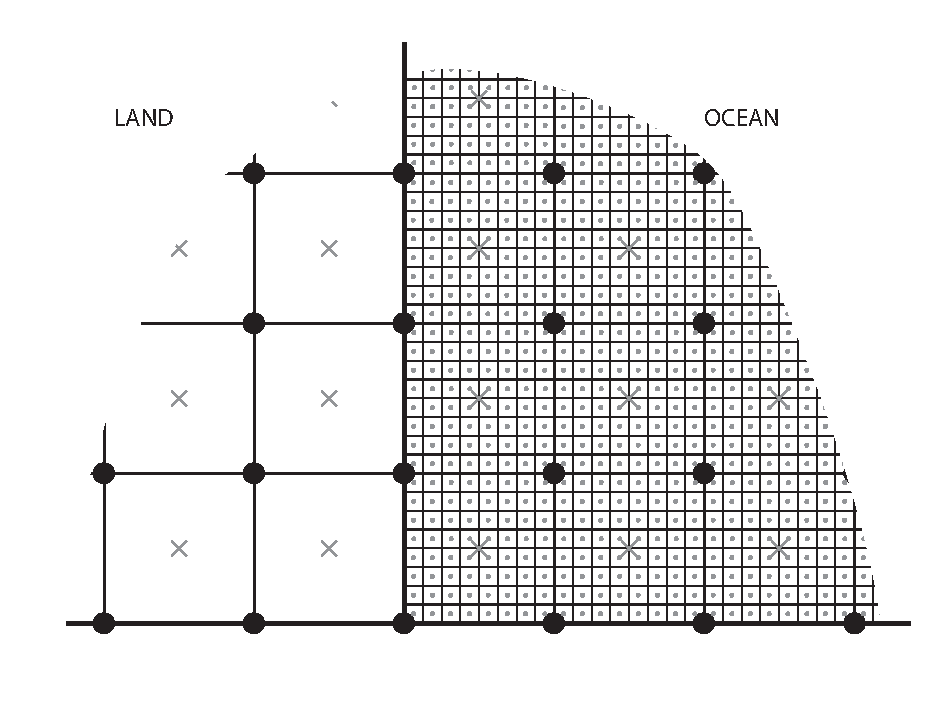
\includegraphics[width=\hsize]{ptgrid}
\caption{\small Cutaway section showing the grid used in the implementation of the model near the land-ocean boundary with 8 ocean gridlengths to every atmosphere gridlength.  The atmosphere grid is the larger grid, with $\bullet$ showing the pressure grid points and $\times$ showing the temperature gridpoints.  The ocean pressure gridpoints are at the vertices of the grid shown, and ocean temperature points indicated by $\cdot$. \label{fig:ptgrid}}
\end{figure}

The advective terms in mixed layer evolution equations such as (\ref{eq:tempdc}), (\ref{eq:hevmatb}) and (\ref{eq:tempcc}) are formulated in the usual manner for C-grid models, in which the advective velocities are computed at the centres of the faces of the cell containing a T gridpoint.
This ensures that the advection scheme is conservative, and that unlike some more sophisticated advection schemes there is no implicit diffusion; it is all explicit.
The quantity being advected is approximated by the average of its values on either side of the face.

The exception to this is the advection of vorticity in equation (\ref{eq:matr1b}).
Here we use a higher order (9-point) Arakawa Jacobian \citep{arakawa:81} with superior conservation properties: it conserves both energy and enstrophy.

The timestepping of the evolution equations uses a leapfrog scheme, which is second order in time.
Occasional averaging of the two time levels carried by the program is performed, to suppress the computational mode which is inevitable with this scheme.


\subsection{Numerical decomposition into modes}\label{sub:modes}
For both ocean and atmosphere the relationship between pressure and vorticity can be written in vector form as in (\ref{eq:matr2b}), where $\mtx{A}$ is the tridiagonal matrix given by (\ref{eq:mata}).
To decompose the layer quantities into modes we suppose that $\mtx{A}$ has left eigenvectors $\vc{L}_m$, right eigenvectors $\vc{R}_m$ and eigenvalues   $\lambda_m$  , where $m$ is the eigenmode number, ranging from 1 to $N$.
Then
\[ \mtx{A} \vc{R}_m  =     \lambda_m\vc{R}_m\]
\[ \vc{L}^T_m  \mtx{A}  =    \lambda_m \vc{L}^T_m\]
for each mode $m$.
It can be shown that $\vc{L}_m$  and $\vc{R}_m$  are orthogonal, i.e $\vc{L}_m^T \cdot \vc{R}_n = 0 $ unless $m = n$.
Note that since $\mtx{A}$ is nonsymmetric  $\vc{L}^T_m \ne \vc{R}_m$   in general.

From the particular structure of $\mtx{A}$, it follows that the eigenvalues will all be real, and for the sign of $\mtx{A}$ chosen in (\ref{eq:matr2a})  $\lambda_m \ge  0$.
The dimensions of    $\lambda_m $   are $1/c_m^2$, where $c_m$  is a phasespeed in m s$^{-1}$.
One of the eigenmodes will have    $\lambda_m $   = 0; we call this the barotropic mode.
We order the remaining $N-1$ modes with $\lambda_m$ increasing ($c_m$ decreasing); these are the baroclinic modes.

The eigenvalues and eigenvectors of $\mtx{A}$ can be computed using standard linear algebra methods \citep[see e.g.][]{golub:83}, and this is done in subroutine \verb=solve_eigenproblem=.
We choose to use routines from the package LAPACK for portability.
We can then use the eigenmodes of $\mtx{A}$ to separate the set of equations (\ref{eq:matr2b})
into an easily soluble set, as follows:

Expand the pressure vector $\vc{p}$ in terms of the right eigenvectors $\vc{R}_n$
\begin{equation}\label{eq:deco1}
\vc{p} = \sum_n \hat{p}_n  \vc{R}_n.
\end{equation}
Premultiply (\ref{eq:deco1}) by $\vc{L}_m^T$, then
\begin{equation}\label{eq:deco2}
\vc{L}_m^T \cdot \vc{p} = \sum_n \hat{p}_n \vc{L}_m^T \vc{R}_n=  \hat{p}_m \vc{L}_m^T \cdot \vc{R}_m,
\end{equation}
by orthogonality, so that
\begin{equation}\label{eq:deco3}
\hat{p}_m = \clm \vc{p} ,
\end{equation}
where $\clm(m,k) = \frac{\vc{L}_m^T (k)}{ \vc{L}_m^T \cdot \vc{R}_m}$ is an $N \times N$ matrix used to  convert from layer to modal amplitudes.

We also require a matrix $\cml$ for converting from modal to layer
amplitudes.
Clearly from (\ref{eq:deco1}) $\cml (k,m) =  \vc{R}_m(k)$.
It follows that the product of the matrices $\cml$ and $\clm$  is the identity matrix, as required for consistency.
Note that  for reasons of runtime efficiency the program carries the transposes of  $\clm$ and $\cml$.

Substitute the expansion (\ref{eq:deco1}) into the vector equation (\ref{eq:matr2b}):
\begin{equation}\label{eq:matr2c}
f_0 [\vc{q} -\Dt{} - \beta(y-y_0) ] =  \nabla_H^2  \sum_m \hat{p}_m  \vc{R}_m  - f_0^2 \sum_m \hat{p}_m  \lambda_m \vc{R}_m,
\end{equation}
where the quantity $f_0^2 \lambda_m$ has dimensions $1/\rdm^2$, where $\rdm$ is a
deformation radius (which is infinite for the barotropic mode).
So we have
\begin{equation}\label{eq:matr2d}
f_0 [\vc{q} -\Dt{} - \beta(y-y_0)  ] =  \sum_m \left(\nabla_H^2   - \frac{1}{\rdm^2} \right) \hat{p}_m \vc{R}_m.
\end{equation}
Premultiplying by $\vc{L}^T_k$, summing over the layers ($k$), and dividing by the dot product, we obtain the equation for the amplitude of each mode:
\begin{equation}\label{eq:matr2e}
\left(\nabla_H^2   - \frac{1}{\rdm^2} \right) \hat{p}_m = f_0 \sum_k \clm(m,k) [q_k -\tilde{D}_k - \beta(y-y_0) ].
\end{equation}
So we need to solve a two-dimensional modified Helmholtz equation with a known RHS for each modal amplitude $\hat{p}_m$, using the method given in section \ref{sub:helm}, and convert these to layer amplitudes using (\ref{eq:deco1}).


\subsection{Integration routines}
Several of the radiative flux coefficients introduced in section \ref{sub:rad} involve vertical integrals over the appropriate layers.
A subroutine \verb=trapin= is provided which computes the extended trapezoidal rule approximation to the integral of a tabulated function \citep{press:92}.
Two routines, \verb=xintt= and \verb=xintp=, are provided for computing area integrals.
\verb=xintt= computes the area integral of a quantity tabulated at T points, as a simple sum.
\verb=xintp= computes the area integral of a quantity tabulated at p points.

\subsection{Diffusive timescales}
Several of the equations contain diffusive terms of second or fourth order (recall that the $\nabla_H^6$ term in (\ref{eq:matr1b}) was originally introduced as fourth order terms in (\ref{eq:momxb},b), and is effectively fourth order since $q \sim \nabla_H^2p$).
To understand the damping effect of the diffusion coefficients, it is useful to derive their associated timescales.

Consider some field $p(x,y)$, and introduce second and fourth order diffusive terms into its evolution equation, with coefficients $A_2$ and $A_4$ respectively, so that
\begin{equation}
\pd{p}{t} = \ldots + A_2\nabla_H^2 p - A_4\nabla_H^4p.
\end{equation}
We will require $A_2 , A_4 > 0$  to ensure decay.
Expand $p$ as a two-dimensional Fourier transform:
\begin{equation}
p(x,y) = \sum_k \sum_l \tilde{p}_{kl} e^{ 2 \pi i( kx + ly )}
\end{equation}
then, differentiating the Fourier expansion, we find that each term will cause exponential decay of the coefficient $\tilde{p}_{kl}$, with timescales $\tau_2$, $\tau_4$ given in the finite difference case (using (\ref{eq:four4})) by
\begin{equation}
\frac{1}{\tau_2} =  A_2 \left(  \left[\frac{2 sin(\pi k \delta)}{\delta}\right]^2 + \left[\frac{2 sin(\pi l \delta)}{\delta}\right]^2 \right)
\end{equation}
\begin{equation}
\frac{1}{\tau_4} =  A_4 \left(  \left[\frac{2 sin(\pi k \delta)}{\delta}\right]^2 + \left[ \frac{2 sin(\pi l \delta)}{\delta}\right]^2 \right)^2,
\end{equation}
where $\delta$ is the (equal) gridlength in either direction.
Subroutine \verb=diffts= evaluates these timescales for two special cases:
\begin{enumerate}
\item A circular eddy whose radius is the baroclinic Rossby radius $\rdm$, so $k = l = \frac{1}{2\rdm}$,
\begin{equation}
\frac{1}{\tau^{\textrm{eddy}}_2} =  2 A_2 \left( \frac{2 sin(\pi \delta/2\rdm)}{\delta}\right)^2
\end{equation}
\begin{equation}
\frac{1}{\tau^{\textrm{eddy}}_4} =  4 A_4 \left( \frac{2 sin(\pi \delta/2\rdm)}{\delta}\right)^4
\end{equation}
\item A one-dimensional wave at the highest wavenumber representable on the grid (two gridpoint noise), $k = \frac{1}{2\delta}$, $l = 0$
\begin{equation}
\frac{1}{\tau^{\textrm{grid}}_2} =  A_2 \left( \frac{ 2}{\delta} \right)^2
\end{equation}
\begin{equation}
\frac{1}{\tau^{\textrm{grid}}_4} =  A_4 \left( \frac{ 2}{\delta} \right)^4
\end{equation}
\end{enumerate}


\subsection{Changes Log}
\subsubsection{Changes from v1.3.1 to v1.4.0}
\begin{itemize}
\item Altered mixed layer stress formulation following \cite{duhaut:06} (entails the introduction of bicubic interpolation for velocities).
\item Improved warning messages in case of NetCDF problems.
\item Revised directory structure in model distribution.
\end{itemize}

\subsubsection{Changes from v1.3 to v1.3.1}
\begin{itemize}
  \item More thorough application of \verb=#ifndef atmos_only=, \verb=#ifndef ocean_only= preprocessor flags to remove unnecessary code and common blocks.   Consequent changes include splitting common blocks for covariance and time averages into atmosphere and ocean components, and that atmospheric \verb=*.f= files have been changed to \verb=*.F= files.
\item Simplified preprocessor structure in code.
\item Addition of \verb=wekpo= and its boundary integrals to time averaged fields.
\item Additional ocean zonal transport diagnostics.
\item Modified \verb=Makefile= to more cleanly remove netCDF where required.
\item Extra preprocessor flag \verb=get_areav= to turn area averaging on.
\item Modified format statements to allow up to 9 layers.
\item More checking of input netCDF topography.
\item Better output from validity checking routine.
\item Additional memory diagnostics in \verb=openqg.F=.
\end{itemize}
  
\subsubsection{Changes from v1.2 to v1.3}
\begin{itemize}
  \item Option of channel ocean, which entails new array dimensioning (\verb=nxta=/\verb=nxpa=), redimensioning some atmospheric arrays, changes to \verb=bilint= in \verb=xfosubs.F= and additional code changes as indicated by \verb=#ifdef cyclic_ocean=.
  \item Redefinition of $f_0$ relative to the central latitude of the domain.
  \item New method of computing $\ek{o}$, by interpolation of $\ek{a}$ (rather than from the curl of $\tx{o}{}$).
  \item New method of reading physical parameters (avoids recompilation).
  \item All routines deriving vorticity from pressure are collected in \verb=vorsubs.F=.
  \item Computation of diffusive timescales moved into new subroutine \verb=diffts=.
  \item More use of \verb=#ifdefs= to remove unnecessary computations in particular configurations.
  \item Added \verb=#ifdef= flags \verb=nb_hflux= and   \verb=sb_hflux= to allow easy switching between temperature boundary conditions and hemispheres.
\end{itemize}
\subsubsection{Changes from v1.1 to v1.2}
\begin{itemize}
\item Addition of $\nabla_H^2$ viscosity in the ocean.
\item Addition of $\nabla_H^4$ diffusion in SST and AST.
\item Non-dimensionalising the mixed boundary condition coefficient.
\item Generalisation of atmosphere from 2 layers to $N$ layers.
\item Simplification of atmospheric radiation scheme.
\item Addition of a minimum mixed layer thickness to the atmospheric mixed layer scheme.
\item Added vorticity and Ekman pumping to time-average diagnostics. Added mean outgoing longwave radiation, mean pressure and potential vorticity to monitoring diagnostics.
\item Addition of topography to both atmosphere and ocean  components of the model.
\item More explicit parallelisation for improved performance.
\item More use of \verb=#ifdef=s to reduce wasted data output in uncoupled simulations.
\item Alterations to the structure which move more subroutines into separate \verb=*.f/*.F= files, and shorten the main \verb=openqg.F= file.
\item Addition of \verb=#ifdef small_local= flag to fix problems which arise on machines with a small predefined stacklimit.
\end{itemize}

\subsubsection*{Acknowledgements}
Neil Stringfellow of Manchester Computing assisted with optimisation and parallelisation of the code.
Peter Challenor assisted us to implement the statistics packages which are built into the code.

\section{Helmholtz Solver}

Most of the equations which constitute the model define one variable explicitly in terms of other variables or their derivatives.
The exceptions are the modified Helmholtz equations (\ref{eq:matr2e}) which define pressures \emph{implicitly} in terms of vorticities, subject to suitable boundary conditions.
We require a computationally efficient solution method for such equations.
Write the general inhomogeneous Helmholtz equation as
\begin{equation}\label{eq:helm}
\left(\nabla_H^2 - \frac{1}{\rdm^2}\right) p = Q
\end{equation}
where the right hand side $ Q(x,y)$ is a known function and $\rdm$ is the Rossby radius for a given mode.
The barotropic mode is a special case for which $\rdm$ is infinite, and (\ref{eq:helm}) reduces to Poisson's equation.

We will consider the solution to (\ref{eq:helm}) in a channel periodic in $x$ (the atmospheric and cyclic ocean cases).
The method carries over to the finite box ocean with simple modifications to be discussed later.
Assume the pressure $p(x,y)$ and the right hand side $ Q(x,y)$ are tabulated on a regular grid at positions $x_i = (i-1)dx$  ($M$ points),  $y_j = y_s + (j-1)dy$ ($N$ points), so that $ Q$ is an $M \times N$ matrix $ Q_{ij}$.
Expand $p$ and $ Q$ as one-dimensional Fourier series in the $x$-direction at each of the ($N-2$) values $y_j$ within the domain (i.e. not including the zonal boundaries $j=1$ and $j=N$):
\begin{equation}\label{eq:four6}
p_{ij} = \sum_k \tilde{p}_{k,j} e^{2\pi i k x_i}.
\end{equation}
We can use a Fast Fourier Transform (FFT) routine to efficiently compute the array of coefficients $\tilde{ Q}_{k,j}$ from the known $ Q_{ij}$.
The particular ordering of the values of $k$ in the transform vector depends on the FFT package used, so we ignore such details in this general account.


\subsection{Effect of the Laplacian operator on a Fourier component}\label{sub:four}
This section considers the effect of the $\ps{}{x}$ operator on a single Fourier component.
Consider a one-dimensional Fourier expansion (the extension to two dimensions is straightforward):
\begin{equation}\label{eq:four}p(x) = \sum_k \tilde{p}_k e^{2\pi i k x}.
\end{equation}
In the continuous case, applying the second derivative operator gives
\begin{equation}\label{eq:four2}
\ns{p}{x} = \sum_k - \tilde{p}_k  (2\pi k)^2 e^{2\pi i k x}.
\end{equation}
In the finite difference case, $\ns{p}{x}$ at $x$ is given by the centred-difference approximation
\begin{equation}\label{eq:four3}
\ns{p}{x} = \frac{p(x+dx) - 2 p(x) + p(x-dx)}{dx^2}.
\end{equation}where $dx$ is the gridspacing.
Substituting (\ref{eq:four}) and simplifying somewhat gives\begin{equation}
\ns{p}{x} =\sum_k \tilde{p}_k  \left(\frac{e^{2\pi i k dx} + e^{-2\pi i k dx} -2}{dx^2}\right) e^{2\pi i k x},
\end{equation}
i.e.
\begin{equation}
\ns{p}{x} =\sum_k \tilde{p}_k  \left(\frac{2 cos(2\pi k dx) -2 } {dx^2}\right)e^{2\pi i k x},
\end{equation}
which, using some familiar trigonometric identities, reduces to:
\begin{equation}\label{eq:four4}
\ns{p}{x} =  \sum_k -\tilde{p}_k  \left(\frac{2 sin(\pi k dx) }{dx}\right)^2e^{2\pi i k x}.
\end{equation}
So the finite difference result (\ref{eq:four4}) is similar to the continuous result (\ref{eq:four2}), but with the replacement
\begin{equation}\label{eq:to}
\pi k \Rightarrow \frac{sin(\pi k dx)}{dx},
\end{equation}
in the Fourier coefficient.
For small $k$ (well-resolved wavelengths) these are equivalent.


\subsection{Solution of the modified Helmholtz equation}\label{sub:helm}

Then from (\ref{eq:four4})
\begin{equation}
\ps{p_{ij}}{x} = \sum_k -\tilde{p}_{k,j}  \left(\frac{2 sin(\pi k dx)}{dx}\right)^2e^{2\pi i k x_i}.
\end{equation}
$\ps{p_{ij}}{y}$ at $y = y_j$ is given by the usual centred difference approximation (\ref{eq:four3})
\begin{equation}
\ps{p_{ij}}{y} = \sum_k \left( \frac{\tilde{p}_{k,j+1} - 2\tilde{p}_{k,j} + \tilde{p}_{k,j-1}}{dy^2}\right) e^{2\pi i k x_i}
\end{equation}
so at each internal point $i,j$ we have an equation of the form
\begin{multline}
\sum_k -\tilde{p}_{k,j} \left( \left(\frac{2 sin(\pi k dx)}{dx}\right)^2 + \frac{1}{\rdm^2} \right)e^{2\pi i k x_i}  + \sum_k \left( \frac{\tilde{p}_{k,j+1} - 2\tilde{p}_{k,j} + \tilde{p}_{k,j-1}}{dy^2}\right) e^{2\pi i k x_i}  \\
= \sum_k \tilde{ Q}_{k,j} e^{2\pi i k x_i} .
\end{multline}
But for this to be true at all the points $x = x_i$, it must be true for each Fourier component $e^{2\pi i k x} $ separately, i.e. for all $k$ and $j$, we must have
\begin{equation}\label{eq:four5}
-\tilde{p}_{k,j} \left( \left(\frac{2 sin(\pi k dx)}{dx}\right)^2 + \frac{1}{\rdm^2} \right) + \frac{ \left( \tilde{p}_{k,j+1} - 2\tilde{p}_{k,j} + \tilde{p}_{k,j-1}\right)}{dy^2} = \tilde{ Q}_{k,j}.
\end{equation}
For each value of the $M$ values of $k$, we can thus write the set of ($N-2$) equations (\ref{eq:four5}) for the range of internal $j$ values as a single tridiagonal matrix equation of size $(N-2) \times (N-2)$ relating the unknown vector $\tilde{p}_{k,j}$ and the known vector $\tilde{ Q}_{k,j}$:
\begin{equation}
\left[ \begin{array}{ccccccccccccc}
\cdot & \cdot& & &\\
\cdot & \cdot& \cdot& &\\
 & \cdot & \cdot& \cdot& &\\
 &  & \cdot & \cdot& \cdot& &\\
\\
 &  & & & a & b_k & a & \\
 & &  & & & a & b_k & a & \\
 & & & & & & a & b_k & a & \\
\\
& & & & & & & & \cdot & \cdot& \cdot& &\\
& & & & & & & & & \cdot & \cdot& \cdot&\\
& & & & & & & & &  & \cdot & \cdot& \cdot\\
& & & & & & & & &  & & \cdot & \cdot
\end{array}\right] \tilde{p}_{k,j} = \tilde{ Q}_{k,j}
\end{equation}
where dots denote non-zero coefficients, and the $a$ and $b$ coefficients are known:
\begin{equation}\label{eq:dy2}
a = \frac{1}{dy^2},
\end{equation}
\begin{equation}\label{eq:bk}
 b_k = - \left( \left( \frac{2 sin(\pi k dx)}{dx} \right)^2 + \frac{1}{\rdm^2}\right) - 2a
\end{equation}
Note that to maintain strictly tridiagonal form, only two entries appear on the top and bottom rows of the matrix.
This is equivalent to asserting that $\tilde{p}$ vanishes on the zonal boundaries $j=1$ and $j=N$ for all $k$, and thus $p=0$ also.

Such a tridiagonal system can be efficiently solved for the unknown vector without a full matrix inversion; see any good numerical linear algebra textbook, such as \citet{press:92}.
For the modified Helmholtz operator, it is clear from (\ref{eq:dy2}) and (\ref{eq:bk}) that $|b_k| \ge 2|a| > 0$ for all $k$, so the matrix is ``diagonally dominant'', and no problems of zero pivots can occur.
The tridiagonal method is accurate to about machine precision, without any need for further iterative improvement. 
Having solved the system for $\tilde{p}_{k,j}$ at all $M$ wavenumbers $k$, we can then use (\ref{eq:four6}) at each latitude to get the pressure $p_{ij}$ at all gridpoints.
Thus we have solved the inhomogeneous Helmholtz equation (\ref{eq:helm}) in a zonally periodic channel, subject to the condition $p = 0$ on the zonal boundaries.

In the case of a finite length (box) ocean, where we require $p$ to be constant around the entire boundary, we use Fourier sine transforms instead of the periodic Fourier transforms, to ensure that $p = 0$ on the meridional boundaries too.

Note that the various Fourier transform routines use a significant fraction of the total CPU time.
It is therefore important that the parameters determining the transform lengths should be chosen to have numerous small prime factors, so as to maximise the efficiency of the transform routines.

\subsection{Generating homogeneous solutions}

We can also use this scheme to solve the homogeneous Helmholtz equation for baroclinic modes.
The homogeneous equation is:
\begin{equation}\label{eq:helm1}
\left(\nabla_H^2- \frac{1}{\rdm^2} \right) p = 0.
\end{equation}
Write $p = \mathcal{L} + \frac{s}{\rdm^2}$, where $\mathcal{L}$ is a known solution of Laplace's equation $\nabla_H^2 \mathcal{L} = 0$ which is non-zero on the boundaries; then $s$ satisfies
\begin{equation}\label{eq:helm2}
\left(\nabla_H^2- \frac{1}{\rdm^2} \right) s = \mathcal{L},
\end{equation}
which is of the same form as (\ref{eq:helm}).
$s$ satisfies the usual condition $s = 0$ on the solid boundaries of the domain, so $p = \mathcal{L}$ on these boundaries.
We can add any multiple of these homogeneous solutions to the inhomogeneous solution to obtain any required value of $p$ on the solid boundaries.


\newpage

\appendix

\section{Writing radiation as a perturbation to mean state}\label{app:rad}

\subsection{Functional form of radiation parameters}
We follow a simplified, linearised model of vertical radiative heat transfer in the atmosphere \citep[see][for details on the basics of radiative balance]{peixoto:92}.
At any point in the atmosphere transfer is due to two sources: (i)  blackbody radiative emission from radiatively active elements within the current layer, which is of the form
\[ \textrm{Flux} = \int B(z) \tau_z(z,Z) \, dz\]
and (ii) radiation from other layers which is partially absorbed within the current layer
\[ \textrm{Flux} = F_{\textrm{in}}\tau(Z_{k-1},Z_{k}).\]
Here we have used a new notation $Z_k$ for the unperturbed interface height coordinate (as the model is framed in terms of layer thicknesses) and introduced the transmissivity $\tau$ which is written as
\begin{equation}
\tau(z,Z) = e^{-\frac{Z-z}{z_0}},
\end{equation}
where $\tau(z,Z)$ is the fraction of radiation from $z$ reaching $Z$, and $z_0$ is the (constant) optical depth of the layer (or $\tau(Z,z)$ is the fraction reaching $Z$ from $z$ for downgoing radiation).
Derivatives of the transmissivities are then
\begin{equation}
\tau_z(z,Z) = \frac{\tau(z,Z)}{z_0}.
\end{equation}
In a comprehensive model, the optical depth $z_0$ will vary with height.
We assume for our model that we know the optical depth in each QG layer ($z_k$).
Note also that we use an optical depth of zero at the bottom of the mixed layer, and $z_m$ near the top of the mixed layer.

We have also used the blackbody radiation emitted from each layer which is written according to the Stefan-Boltzmann law
\begin{equation}
\B{m}(z) = \frac{\sigma}{2}(\overline{\T{a}{m}}  + \T{a}{m}' - \gamma z)^4,
\end{equation}
for the mixed layer, and
\begin{equation}
\B{k}(z) = \frac{\sigma}{2}(\T{a}{k} - \gamma z)^4,
\end{equation}
for other layers.
The terms in the temperature function represent constant potential temperature, the variation of in situ temperature with height being determined by the adiabatic lapse rate $\gamma$.

\subsection{Rules for linearising}
We want to linearise the radiation equations about a mean state.
To do this we expand about a mean and retain the first order terms in $\T{a}{m}'$, $\etb{a}{m}$ and $\etb{a}{k}$.
Note that the topography $\D{a}$ is included as a first order perturbation to the radiation, as it is to the dynamics.
It therefore does not enter the mean state calculation.
For the mixed layer radiation function
\begin{equation}
\frac{\sigma}{2}(\overline{\T{a}{m}} - \gamma z + \T{a}{m}')^4 \approx \frac{\sigma}{2}(\overline{\T{a}{m}} - \gamma z)^4 + 2\sigma(\overline{\T{a}{m}} - \gamma z)^3 \, \T{a}{m}'.
\end{equation}

Transmissivities are expanded by writing, for example,
\begin{equation}
\begin{split}
\tau(\h{a}{m}+\D{a},\h{a}{1}) &= e^{-\frac{\Z{a}{1} + \etb{a}{1} -\HH{a}{m} -\D{a} - \etb{a}{m}}{z_1}} \\
&= e^{-\frac{\Z{a}{1} -\HH{a}{m}}{z_1}} e^{-\frac{\etb{a}{1}}{z_1}}e^{\frac{\etb{a}{m}+\D{a}}{z_1}}\\
&\approx \tau_1\left(1 -  \frac{\etb{a}{1}}{z_1} \right)\left(1 + \frac{\etb{a}{m}+\D{a}}{z_1} \right)\\
&\approx \tau_1\left(1 -  \frac{\etb{a}{1}}{z_1}  + \frac{\etb{a}{m}+\D{a}}{z_1} \right)
\end{split}
\end{equation}
where $\tau_1 \equiv e^{-\frac{\Z{a}{1}-\HH{a}{m} }{z_1}}$ is the unperturbed value.
For other layers, $\tau_k \equiv e^{-\frac{\HH{a}{k}}{z_k}}$.

Any integrals are also linearised as, for example,
\begin{equation}
\int_{\h{a}{m} + \D{a} }^{\Z{a}{1} + \etb{a}{1}}f(z)dz \approx \int_{\HH{a}{m} }^{\Z{a}{1}}f(z)dz - f(\HH{a}{m}) (\etb{a}{m}+\D{a}) + f(\Z{a}{1}) \etb{a}{1}.
\end{equation}

When calculating the radiation at any point, we write the full radiation balance, first expand the integration and then expand remaining terms, eliminating quadratic and higher order terms.
This is explicitly done for each layer in the following section.

\subsection{Calculations}

\begin{description}

\item[Oceanic Mixed Layer] absorbs all downgoing longwave radiation (as well as incoming shortwave radiation) which passes through the atmospheric mixed layer.
Emits radiation according to its blackbody temperature,
\begin{equation}
\Fup{0} = \B{0}(0) = \sigma \left(\overline{\T{o}{m}} + \T{o}{m}'\right)^4.
\end{equation}
We linearise this by writing
\begin{equation}
\Fup{0} \approx \overline{\Fup{0}} + \dup{0}\T{o}{m}'
\end{equation}
where
\begin{equation}
\overline{\Fup{0}} = \sigma \overline{\T{o}{m}}^4,
\end{equation}
\begin{equation}
\dup{0} = 4\sigma \overline{\T{o}{m}}^3.
\end{equation}

\item[Atmospheric Mixed Layer]

To calculate upward radiation leaving the atmospheric mixed layer, we note that optical depth at the base of the mixed layer is assumed to be zero: thus outgoing radiation here must be internally generated:
\begin{equation}
\Fup{m} = \int_{\D{a}}^{\h{a}{m}+\D{a}} \B{m}(z) {\tau_z(z,\h{a}{m}+\D{a})} \, dz.
\end{equation}
We first linearise the integral, giving
\begin{multline}
\Fup{m} \approx \int_0^{\HH{a}{m}} \B{m}(z) {\tau_z(z,\h{a}{m})} \,dz + \B{m}(\HH{a}{m}) {\tau_z(\HH{a}{m} ,\h{a}{m}+\D{a})}(\etb{a}{m}+\D{a}) - \\
\B{m}(0) \tau_z(0,\h{a}{m}+\D{a})\D{a},
\end{multline}
and then evaluate each of the terms (noting that the last term disappears because the mixed layer is opaque at the bottom),
\begin{multline}
\Fup{m} \approx \int_0^{ \HH{a}{m} } \left(\frac{\sigma}{2}(\overline{\T{a}{m}} - \gamma z)^4 + 2\sigma \left(\overline{\T{a}{m}} - \gamma z\right)^3\T{a}{m}'\right) \frac{e^{-\frac{\HH{a}{m} - z}{z_m}}}{z_m}\left(1 - \frac{\etb{a}{m}+\D{a}}{z_m}\right)  \,dz \\
+ \frac{\sigma}{2} \left(\overline{\T{a}{m}} - \gamma \HH{a}{m} \right)^4 \frac{\etb{a}{m}+\D{a}}{z_m} .
\end{multline}
By omitting the remaining quadratic terms we obtain an expression for upwards radiation,
\begin{multline}
\Fup{m} \approx \frac{\sigma \iup{m}}{2 z_m} + \left(\frac{2\sigma}{z_m} \int_0^{ \HH{a}{m} } \left( \overline{ \T{a}{m} } - \gamma z \right)^3 e^{ - \frac{ \HH{a}{m} - z }{ z_m } } \,dz \right)  \T{a}{m}' \\
+ \left(\frac{\sigma}{2 z_m}(\overline{\T{a}{m}} - \gamma \HH{a}{m} )^4  - \frac{\sigma \iup{m}}{2 {z_m}^2}\right)(\etb{a}{m}+\D{a}) .
\end{multline}
Here we have defined
\[\iup{m} = \int_0^{ \HH{a}{m} } \left(\overline{\T{a}{m}} - \gamma z\right)^4 e^{-\frac{\HH{a}{m}- z}{z_m}}  \,dz,\]
and we use similar integrals when calculating radiation in other layers.
The complete radiation formula is written in terms of the coefficients
\begin{equation}
\overline{\Fup{m}} = \frac{\sigma\iup{m}}{2 z_m},
\end{equation}
\begin{equation}
 \bup{m} =\left( \frac{\sigma}{2}(\overline{\T{a}{m}} - \gamma \HH{a}{m})^4  - \overline{\Fup{m}}\right) \frac{1}{ z_m} ,
\end{equation}
\begin{equation}
 \cupp{m} =\bup{m},
\end{equation}
\begin{equation}
\dup{m} = \frac{ 2 \sigma }{ z_m } \int_0^{ \HH{a}{m} } \left( \overline{ \T{a}{m} } - \gamma z\right)^3 e^{-\frac{ \HH{a}{m} - z }{ z_m }} \,dz,
\end{equation}
giving
\begin{equation}
\Fup{m} \approx \overline{\Fup{m}} + \bup{m} \etb{a}{m} + \cupp{m} \D{a} + \dup{m} \T{a}{m}'.
\end{equation}
These constant coefficients are evaluated at the initialisation of the model, and stored for later use.

Downgoing radiation can be calculated simply using the assumption that optical depth at the bottom of the mixed layer is $z_0 = 0$, so that radiation only depends upon local temperature,
\begin{equation} \begin{split}
\Fdown{m} & \approx -\frac{\sigma }{2} \overline{ \T{a}{m} }^4 - 2 \sigma \overline{ \T{a}{m} }^3 \T{a}{m}' \\
& = \overline{\Fdown{m}} + \ddown{m}\T{a}{m}',
\end{split}\end{equation}
where
\begin{equation}
\overline{\Fdown{m}} = - \frac{\sigma}{2} \overline{ \T{a}{m} }^4,
\end{equation}
\begin{equation}
\ddown{m} = - 2\sigma \overline{ \T{a}{m} }^3.
\end{equation}

\item[Atmospheric QG layers]

The QG layers include both partial absorption and emission terms,
\begin{equation}\label{eq:fluxn}
\Fup{k} = \Fup{k-1} \tau(\Z{a}{k-1}+\etb{a}{k-1},\Z{a}{k}+\etb{a}{k}) + \int_{\Z{a}{k-1}+\etb{a}{k-1}}^{\Z{a}{k}+\etb{a}{k}} \B{k}(z) {\tau_z(z,\Z{a}{k}+\etb{a}{k})} \, dz.
\end{equation}
Note that when $k=1$, we use $\Z{a}{k-1} = \HH{a}{m}$ and $\etb{a}{k-1} = \etb{a}{m} + \D{a}$.
The full equation is thus
\begin{multline}
\Fup{k} =  \left(\overline{\Fup{k-1}} + \Fup{k-1}^{\prime}\right) \tau_k \left(1 + \frac{\etb{a}{k-1}}{z_k} - \frac{\etb{a}{k}}{z_k}\right)  \\
+ \int_{\Z{a}{k-1}}^{\Z{a}{k}} \frac{\sigma}{2}(\T{a}{k} - \gamma z)^4  \frac{e^{-\frac{\Z{a}{k}- z }{z_k}}}{z_k} \left( 1 - \frac{\etb{a}{k}}{z_k}\right) \, dz \\
-  \frac{\sigma}{2}(\T{a}{k} - \gamma \Z{a}{k-1})^4 \frac{\tau_k}{z_k} \etb{a}{k-1} +  \frac{\sigma}{2}(\T{a}{k} - \gamma \Z{a}{k})^4 \frac{\etb{a}{k}}{z_k}.
\end{multline}
Again we organise this equation into mean and perturbation quantities,
\begin{multline}
\Fup{k} \approx \overline{\Fup{k-1}}\tau_k + \frac{\sigma \iup{k}}{2 z_k} + \Fup{k-1}^{\prime} \tau_k + \left(\overline{\Fup{k-1}} - \frac{\sigma}{2}(\T{a}{k} - \gamma \Z{a}{k-1})^4\right) \frac{\tau_k}{z_k} \etb{a}{k-1}\\
+ \left( - \overline{\Fup{k-1}} \tau_k - \frac{\sigma \iup{k}}{2 z_k}+  \frac{\sigma}{2}(\T{a}{k} - \gamma \Z{a}{k})^4  \right) \frac{\etb{a}{k}}{z_k},
\end{multline}
where
\[\iup{k} = \int_{\Z{a}{k-1}}^{\Z{a}{k}} \left(\overline{\T{a}{k}} - \gamma z\right)^4 e^{-\frac{\Z{a}{k}- z}{z_k}} \,dz.\]
Note that this equation requires contributions from layers below so that the individual terms need to be evaluated from the bottom upwards.
The general form of the equation is
\begin{equation}
\Fup{k} \approx \overline{\Fup{k}} + \sum_{i=1}^{\textrm{min}(k,N-1)}\aup{k,i}\etb{a}{i} + \bup{k} \etb{a}{m} + \cupp{k} \D{a} + \dup{k}\T{a}{m}'\quad \quad \textrm{for }k=1,N,
\end{equation}
where
\begin{equation}
\overline{\Fup{k}} =\overline{\Fup{k-1}}\tau_k + \frac{\sigma \iup{k}}{2 z_k} ,
\end{equation}
\begin{equation}
\dup{1} = \dup{m} \tau_1,
\end{equation}
\begin{equation}
\dup{k} = \dup{k-1} \tau_k \quad \quad \textrm{for }k=2,N.
\end{equation}
Calculation of the other three terms is more complicated:
\begin{equation}
\bup{1} =  \left(\bup{m} + \frac{ \overline{ \Fup{m} } }{ z_1 } - \frac{ \sigma }{ 2 z_1} ( \T{a}{1} - \gamma \HH{a}{m} )^4 \right) \tau_1,
\end{equation}
\begin{equation}
\bup{k} =  \bup{k-1} \tau_k \quad \quad \textrm{for }k=2,N.
\end{equation}
\begin{equation}
\cupp{1} =  \left(\cupp{m} + \frac{ \overline{ \Fup{m} } }{ z_1 } - \frac{ \sigma }{ 2 z_1} ( \T{a}{1} - \gamma \HH{a}{m} )^4 \right) \tau_1,
\end{equation}
\begin{equation}
\cupp{k} =  \cupp{k-1} \tau_k \quad \quad \textrm{for }k=2,N.
\end{equation}
\begin{equation}
\aup{1,1} = \left( - \overline{\Fup{m}} \tau_1 - \frac{\sigma \iup{1}}{2 z_1}+  \frac{\sigma}{2}(\T{a}{1} - \gamma \Z{a}{1})^4\right) \frac{1}{z_1},
\end{equation}
\begin{equation}
\aup{k,k} = \left(  - \overline{\Fup{k-1}} \tau_k - \frac{\sigma \iup{k}}{2 z_k}+  \frac{\sigma}{2}(\T{a}{k} - \gamma \Z{a}{k})^4\right) \frac{1}{z_k} \quad \quad \textrm{for }k = 2,N-1,
\end{equation}
\begin{equation}
\aup{k,k-1} = \left(\frac{\overline{\Fup{k-1}}}{z_k} + \aup{k-1,k-1} - \frac{\sigma}{2z_k}(\T{a}{k} - \gamma \Z{a}{k-1})^4\right)\tau_k \quad \quad \textrm{for }k = 2,N.
\end{equation}
\begin{equation}
\aup{k,i} = \aup{k-1,i}\tau_k \quad \quad \textrm{for }i =1, k-2 \quad \textrm{and} \quad k=3,N.
\end{equation}

For downgoing radiation the full equation is
\begin{equation}
\Fdown{k} =  \Fdown{k+1}\tau(\Z{a}{k-1}+\etb{a}{k-1},\Z{a}{k}+\etb{a}{k}) + \int_{\Z{a}{k-1}+\etb{a}{k-1}}^{\Z{a}{k}+\etb{a}{k}} \B{k}(z) \tau_z(\Z{a}{k-1}+\etb{a}{k-1},z) \, dz
\end{equation}
which reduces to
\begin{multline}
\Fdown{k} \approx \left( \overline{\Fdown{k+1}} + \Fdown{k+1}^{\prime} \right) \tau_k \left( 1 + \frac{\etb{a}{k-1}}{z_k} - \frac{\etb{a}{k}}{z_k} \right) \\
- \int_{\Z{a}{k-1}}^{\Z{a}{k}} \frac{\sigma}{2}(\T{a}{k} - \gamma z)^4\frac{e^{-\frac{z-\Z{a}{k-1}}{z_k}}}{z_k}\left(1+\frac{\etb{a}{k-1}}{z_k}\right)  \, dz\\
 + \frac{\sigma}{2}(\T{a}{k} - \gamma \Z{a}{k-1})^4\frac{\etb{a}{k-1}}{z_k} - \frac{\sigma}{2}(\T{a}{k} - \gamma \Z{a}{k})^4\frac{\tau_k}{z_k}\etb{a}{k},
\end{multline}
giving
\begin{multline}
\Fdown{k} \approx \overline{\Fdown{k+1}}\tau_k - \frac{\sigma \idown{k}}{2 z_k} + \Fdown{k+1}^{\prime} \tau_k +  \left( \overline{\Fdown{k+1}}\tau_k - \frac{\sigma \idown{k}}{2 z_k} +  \frac{\sigma}{2}(\T{a}{k} - \gamma \Z{a}{k-1})^4\right) \frac{\etb{a}{k-1}}{z_k} \\
+ \left( - \overline{\Fdown{k+1}} - \frac{\sigma}{2}(\T{a}{k} - \gamma \Z{a}{k})^4\right) \frac{\tau_k}{z_k}\etb{a}{k},
\end{multline}
where
\[\idown{k} = \int_{\Z{a}{k-1}}^{\Z{a}{k}} \left(\overline{\T{a}{k}} - \gamma z\right)^4 e^{-\frac{z-\Z{a}{k-1}}{z_k}} \,dz.\]
This equation requires contributions from layers above, so that the individual terms need to be evaluated from the top downwards.
This can be written in the general form
\begin{equation}
\Fdown{k} \approx \overline{\Fdown{k}} + \sum_{i=\max(k-1,1)}^{N-1} \adown{k,i} \etb{a}{i} + \bdown{k} \etb{a}{m} + \cdown{k} \D{a} \quad \quad \textrm{for }k=1,N,
\end{equation}
where we know
\begin{equation}
 \overline{\Fdown{k}} =\overline{\Fdown{k+1}}\tau_k - \frac{\sigma \idown{k}}{2 z_k},
\end{equation}
\begin{equation}
\bdown{1} = \left( \overline{\Fdown{2}}\tau_1 - \frac{\sigma \idown{1}}{2 z_1} +\frac{\sigma}{2}(\T{a}{1} - \gamma \HH{a}{m})^4\right) \frac{1}{z_1} ,
\end{equation}
\begin{equation}
\bdown{k} = 0 \quad \quad \textrm{for }k=2,N,
\end{equation}
\begin{equation}
\cdown{1} = \bdown{1}
\end{equation}
\begin{equation}
\cdown{k} = 0 \quad \quad \textrm{for }k=2,N,
\end{equation}
\begin{equation}
\adown{N,N-1} =  \left( - \frac{\sigma \idown{N}}{2 z_N} +  \frac{\sigma}{2}(\T{a}{N} - \gamma \Z{a}{N-1})^4\right) \frac{1}{z_N} ,
\end{equation}
\begin{equation}
\adown{k,k-1} =  \left( \overline{\Fdown{k+1}}\tau_k - \frac{\sigma \idown{k}}{2 z_k} +  \frac{\sigma}{2}(\T{a}{k} - \gamma \Z{a}{k-1})^4\right) \frac{1}{z_k} \quad \quad \textrm{for }k=2,N-1,
\end{equation}
\begin{equation}
\adown{k,k} =  \left( \adown{k+1,k} - \frac{\overline{\Fdown{k+1}}}{z_k} - \frac{\sigma}{2 z_k}(\T{a}{k} - \gamma \Z{a}{k})^4\right) \tau_k,\quad \quad \textrm{for }k=1,N-1,
\end{equation}
\begin{equation}\label{eq:adownki}
\adown{k,i} =   \adown{k+1,i}\tau_k \quad \quad \textrm{for }k=1,N-1\textrm{ and }i = k+1,N-1,
\end{equation}

\end{description}

\section{Constraints on mass and momentum}

\subsection{Atmospheric momentum constraints}\label{app:atcon}

Following \citet{mcwilliams:77} we need to find constraints on momentum for flow in the channel atmosphere.
We start with an example of using constraints in the continuous case and then progress to the discrete case.

\subsubsection{The continuous case}
To determine these constraints in the continuous case, we integrate as an example the atmospheric layer 1 vorticity from (\ref{eq:matr1b}) over the entire basin area $A$,
\begin{multline}\label{eq:vortint1}
\iint \nabla_H^2\p{a}{1}_t \, dA  - \frac{f_0^2}{\HH{a}{1}}\iint\etb{a}{1}_t \, dA = \iint J(\q{a}{1},\p{a}{1})\, dA  +\\
  \frac{f_0^2}{\HH{a}{1}}\iint (\e{a}{1} - \ek{a}) \, dA - \ah{a} \iint \nabla_H^6 \p{a}{1} \,dA.
\end{multline}
We apply a mass constraint
\begin{equation}
\iint  \etb{a}{1}_t \, dA= - \iint \e{a}{1} \, dA,
\end{equation}
and require that there is no net advection over the basin, giving
\begin{equation}
\iint \nabla_H^2\p{a}{1}_t \, dA =  - \frac{f_0^2}{\HH{a}{1}}\iint  \ek{a} \, dA - \ah{a} \iint \nabla_H^6 \p{a}{1} \, dA.
\end{equation}
This equation can be simplified by writing
\begin{equation}
\iint \nabla_H.(\nabla_H\p{a}{1}_t) \, dA =  - \frac{f_0}{\HH{a}{1}}\iint \nabla_H \times \vc{\tau} \, dA - \ah{a} \iint \nabla_H . \nabla_H(\nabla_H^4 \p{a}{1}) \, dA
\end{equation}
so that application of Gauss' and Stokes' theorems in a periodic channel gives
\begin{equation}  \label{eq:momintd}
\int \left[\p{a}{1}_{yt}\right]_0^{L_y}\, dx = \frac{f_0}{\HH{a}{1}}\int \left[\tx{a}{x}\right]_0^{L_y} \, dx  - \ah{a} \int \left[\nabla_H^4 \p{a}{1}_y\right]_0^{L_y}\, dx,
\end{equation}
where the square brackets refers to the difference between the values of the variables within at the north and south of the domain.
The equivalent equations can be found in other layers in the same way.

\subsubsection{The discrete case}\label{app:discon}
The same equations can be written for the discrete case, however we only know about vorticity evolution at internal points in the domain (and not the boundary points).
Therefore we integrate only over the internal points (area $A_I$)
\begin{multline}\label{eq:momnew}
\iint \nabla_H^2\p{a}{1}_t \, dA_I  - \frac{f_0^2}{\HH{a}{1}}\iint\etb{a}{1}_t \, dA_I = \iint J(\q{a}{1},\p{a}{1})\, dA_I  +\\
 \frac{f_0^2}{\HH{a}{1}}\iint (\e{a}{1} - \ek{a}) \, dA_I - \ah{a} \iint \nabla_H^6 \p{a}{1} \,dA_I
\end{multline}
and note that there remain finite contributions from the advection terms and the mass balance.
The displacement and entrainment terms are simplified using
\begin{multline}\label{eq:etae1}
\iint \left( \etb{a}{1}_t + \e{a}{1} \right) \, dA= \iint \left( \etb{a}{1}_t + \e{a}{1} \right) \, dA_I \\
+ \frac{\Delta y}{2}\int\left[\left( \etb{a}{1}_t + \e{a}{1} \right)^{(1)} + \left( \etb{a}{1}_t + \e{a}{1} \right)^{(n)}\right] \, dx = 0,
\end{multline}
giving
\begin{equation}
\iint \left( \etb{a}{1}_t + \e{a}{1} \right) \, dA_I = - \frac{\Delta y}{2}\int\left[\left( \etb{a}{1}_t + \e{a}{1} \right)^{(1)} + \left( \etb{a}{1}_t + \e{a}{1} \right)^{(n)}\right] \, dx.
\end{equation}
Here the bracketed superscripts refer to the value of the quantity at that gridpoint.

Since the Jacobian describes conservative advection of $q_1$, its integral vanishes over the interior of the domain, leaving contributions only from some near-boundary components.
So we can write
\begin{equation}\label{eq:jacat1}
\iint J(\q{a}{1},\p{a}{1})\, dA_I  = \int\left(J_1^{(1)} + J_1^{(n)} \right) \, dx.
\end{equation}
where $J_k$ is the evaluation of the non-cancelling Jacobian terms near the boundary of layer $k$.

Following \citet{mcwilliams:77} we choose to satisfy constraints along each of the north and south boundaries independently.
We gather all the terms in (\ref{eq:momnew}), once again applying Stokes' and Gauss' theorems to simplify the pressure derivatives and Ekman pumping term, and write two equations for the constraints on the atmospheric layer 1 flow,
\begin{multline}\label{eq:south1}
- \int \p{a}{1}_{yt}^{(1.5)}\, dx  + \frac{f_0^2 \Delta y}{2 \HH{a}{1}}\int \etb{a}{1}_t^{(1)} \, dx \\
=  \int J_1^{(1)}\, dx - \frac{f_0^2 \Delta y}{2 \HH{a}{1}}\int \e{a}{1}^{(1)}\, dx - \frac{f_0}{\HH{a}{1}}\int {\tx{a}{x}}^{(1.5)} \, dx  + \ah{a} \int \p{a}{1}_{5y}^{(1.5)}\, dx,
\end{multline}
\begin{multline}\label{eq:north1}
\int \p{a}{1}_{yt}^{(n-0.5)}\, dx  + \frac{f_0^2 \Delta y}{2 \HH{a}{1}}\int \etb{a}{1}_t^{(n)} \, dx = \int J_1^{(n)}\, dx - \frac{f_0^2 \Delta y}{2 \HH{a}{1}}\int \e{a}{1}^{(n)}\, dx \\
+ \frac{f_0}{\HH{a}{1}}\int {\tx{a}{x}}^{(n-0.5)} \, dx  - \ah{a} \int \p{a}{1}_{5y}^{(n-0.5)}\, dx.
\end{multline}
Note that the integral over internal pressure points gives terms which must be evaluated half a gridpoint in from the boundary (the first and last two terms in the above equations), and that in the upper layer we can simplify the Ekman pumping term using Stokes' theorem (although this distinction is lost in the vector equations below).

These equations can be generalised to the vector form (with the exception of the linear integral of stress in the previous equations), so that the constraints on all layers can be written 
\begin{multline}\label{eq:south2}
- \int \vc{p}_{yt}^{(1.5)}\, dx  + \frac{f_0^2 \Delta y}{2}\mtx{A}\int \vc{p}_t^{(1)} \, dx \\
= \int \vc{J}^{(1)}\, dx + \frac{f_0 \Delta y}{2}\mtx{{}^a B}\int \vc{{}^a e}^{(1)}\, dx  + \ah{a} \int \vc{p}_{5y}^{(1.5)}\, dx,
\end{multline}
\begin{multline}\label{eq:north2}
\int \vc{p}_{yt}^{(n-0.5)}\, dx  + \frac{f_0^2 \Delta y}{2}\mtx{A}\int \vc{p}_t^{(n)} \, dx \\
= \int \vc{J}^{(n)}\, dx + \frac{f_0 \Delta y}{2}\mtx{{}^a B}\int \vc{{}^a e}^{(n)}\, dx  - \ah{a} \int \vc{p}_{5y}^{(n-0.5)}\, dx.
\end{multline}
The right hand sides of (\ref{eq:south2}) and (\ref{eq:north2}) are accumulated in the program during timestepping. Therefore we define
\[\vc{L}^{\textrm S} = - \int \vc{p}_{y}^{(1.5)}\, dx  + \frac{f_0^2 \Delta y}{2}\mtx{A}\int \vc{p}^{(1)} \, dx\]
\[\vc{L}^{\textrm N} =\int \vc{p}_{y}^{(n-0.5)}\, dx  + \frac{f_0^2 \Delta y}{2}\mtx{A}\int \vc{p}^{(n)} \, dx \]
\[\vc{R}^{\textrm S} =  \int \vc{J}^{(1)}\, dx + \frac{f_0 \Delta y}{2}\mtx{{}^a B}\int \vc{{}^a e}^{(1)}\, dx  + \ah{a} \int \vc{p}_{5y}^{(1.5)}\, dx,\]
\[\vc{R}^{\textrm N} =\int \vc{J}^{(n)}\, dx + \frac{f_0 \Delta y}{2}\mtx{{}^a B}\int \vc{{}^a e}^{(n)}\, dx  - \ah{a} \int \vc{p}_{5y}^{(n-0.5)}\, dx.\]
It follows from (\ref{eq:south2}) and (\ref{eq:north2}) that, after timestepping, the new values of $\vc{L}$ can be written
\[\vc{L}_{new} = \vc{L}_{old} + 2 \delta t \vc{R}\]
for both the northern and southern boundaries.

With knowledge of the evolution of $\vc{L}$ at both the north and south boundaries we proceed to solve for pressure using the Helmholtz solver, which returns a modal pressure $\vc{\tilde{p}}$ which is zero on both north and south boundaries.
We are looking for $\vc{\hat{p}}$, the full modal pressure including boundary contributions, which can be written as a linear superposition of $\vc{\tilde{p}}$ and two precomputed solutions to the homogeneous Helmholtz equation:
\[\vc{\hat{p}}(x,y) = \vc{\tilde{p}}(x,y) + \vc{C}_{1}\vc{P}_{1}(y) + \vc{C}_{2}\vc{P}_{2}(y).\]
Note that the precomputed solutions $\vc{P}_{1}$ and $\vc{P}_{2}$ are found from (\ref{eq:helm1}) and (\ref{eq:helm2}) using the linear functions 
\[\mathcal{L}_1(y) = \frac{{}^aY-y}{{}^aY},\] 
and
\[\mathcal{L}_2(y)=\frac{y}{{}^aY}.\] 
We need to solve for coefficient vectors $\vc{C}_{1}$ and  $\vc{C}_{2}$.
To do this we take advantage of the conversion between modal and layer pressures to write
\[\vc{L}^{\textrm S} = - \int \cml \vc{\hat{p}}_{y}^{(1.5)}\, dx  + \frac{f_0^2 \Delta y}{2}\mtx{A}\int \cml \vc{\hat{p}}^{(1)} \, dx,\]
which gives
\begin{multline}
\vc{L}^{\textrm S} = - \cml \int \left( \vc{\tilde{p}}_{y}^{(1.5)} + \vc{C}_{1}\vc{P}_{1y}^{(1.5)} + \vc{C}_{2}\vc{P}_{2y}^{(1.5)} \right) \, dx  + \\
\frac{f_0^2 \Delta y}{2}\mtx{A}\cml \int  \left( \vc{\tilde{p}}^{(1)} + \vc{C}_{1}\vc{P}_{1}^{(1)} + \vc{C}_{2}\vc{P}_{2}^{(1)} \right)  \, dx. \nonumber
\end{multline}
Premultiply by $\clm$,
\begin{multline}
\clm \vc{L}^{\textrm S} =  - \int \left(  \vc{\tilde{p}}_{y}^{(1.5)} + \vc{C}_{1}\vc{P}_{1y}^{(1.5)} + \vc{C}_{2}\vc{P}_{2y}^{(1.5)} \right)  \, dx  +\\
 \frac{f_0^2 \Delta y}{2} \vc{\lambda} \int \left(  \vc{\tilde{p}}^{(1)} + \vc{C}_{1}\vc{P}_{1}^{(1)} + \vc{C}_{2}\vc{P}_{2}^{(1)}  \right) \, dx,\nonumber
\end{multline}
where have used the identities $\clm\cml  = 1$ and $\clm\mtx{A}\cml  = \vc{\lambda}$.
Thus, using the fact that  $\vc{\tilde{p}}^{(1)}$ vanishes on the boundary, we can write
\begin{multline}
\clm \vc{L}^{\textrm S} + \int \vc{\tilde{p}}_{y}^{(1.5)} \, dx =  \vc{C}_{1} \left[ - \int \vc{P}_{1y}^{(1.5)} \, dx +
\frac{f_0^2 \Delta y}{2} \vc{\lambda} \int \vc{P}_{1}^{(1)}  \, dx\right] \\
+  \vc{C}_{2} \left[ - \int \vc{P}_{2y}^{(1.5)} \, dx  + \frac{f_0^2 \Delta y}{2} \vc{\lambda} \int \vc{P}_{2}^{(1)} \, dx \right] .
\end{multline}
Likewise, for the northern boundary we can write
\begin{multline}
\clm \vc{L}^{\textrm N} - \int \vc{\tilde{p}}_{y}^{(n-0.5)} \, dx =  \vc{C}_{1} \left[\int \vc{P}_{1y}^{(n-0.5)} \, dx + \frac{f_0^2 \Delta y}{2} \vc{\lambda} \int \vc{P}_{1}^{(n)}  \, dx\right] \\
+  \vc{C}_{2} \left[\int \vc{P}_{2y}^{(n-0.5)} \, dx  + \frac{f_0^2 \Delta y}{2} \vc{\lambda} \int \vc{P}_{2}^{(n)} \, dx \right] .
\end{multline}
Thus we have a pair of simultaneous linear equations for the homogeneous solution coefficients $\vc{C}_{1}$ and  $\vc{C}_{2}$.
The terms in the square brackets can be precomputed at model initialisation (in subroutine \verb=homsol=); the left hand sides are determined at each timestep, and  $\vc{C}_{1}$ and  $\vc{C}_{2}$ are then found.
These are used to form the baroclinic modes, and the modes are transformed into layer pressures using the matrix $\cml$.

The barotropic mode is a special case of the above, because the eigenvalue $\lambda_b$ is zero.
In addition, according to \citet{mcwilliams:77} we need only one constraint on the barotropic mode; we choose to apply this on the southern boundary.
In addition we only have one homogeneous barotropic mode (as the barotropic mode satisfies $p_{yy}=0$).
The equations then reduce to
\[\left(\clm \vc{L}^{\textrm S} + \int \vc{\tilde{p}}_{y}^{(1.5)} \, dx\right)_b =  - C_{b} \int {P_{b}}_{y}^{(1.5)} \, dx  ,\]
where we have chosen $P_b = 1-\tfrac{y}{{}^aY}$, and thus can explicitly write
\[C_{b} =  \frac{{}^aY}{{}^aX}\left(\clm \vc{L}^{\textrm S} + \int \vc{\tilde{p}}_{y}^{(1.5)} \, dx\right)_b.\]

We perform a consistency check on the conservation of mass in the baroclinic solutions.
The change in mean interface height between timesteps can be explicitly calculated from the integral of entrainment.
This is compared with the change computed by applying the constaints  derived above, and the absolute and fractional errors are stored in the monitoring variables \verb=ermas= and \verb=emfr=.


\subsection{Ocean constraints}\label{app:occon}

\subsubsection{Box ocean case}\label{app:boxcon}

At each interface $k$ we have a mass constraint
\begin{equation}\label{eq:occon2}
\iint \etb{o}{k}_t \, dA =  - \iint \e{o}{k}\, dA, \quad\quad k = 1,N-1.
\end{equation}
The pressures obtained by solving the inhomogeneous Helmholtz equations will not necessarily satisfy these constraints; this is achieved by adding suitable multiples of the homogeneous solutions.

Although we have posed the constraints quite generally, we in practice make a very restrictive choice of allowed entrainment.
We choose entrainment in the ocean to act only on the uppermost interface, so that $\e{o}{k}\equiv0$ for $k=2,N-1$ (see \ref{eq:eok1}).
At interface 1, entrainment is nonzero.
However (\ref{eq:occon2}), as well as ensuring conservation of mass, also determines the amount of heat entering the deep ocean.
As OpenQG has no overturning circulation or vertical diffusion, there is no mechanism for heat to be transferred from the deep ocean back to the surface layer.
Therefore, we adjust (in subroutine \verb=oml=) the entrainment $\e{o}{1}$ to satisfy 
\begin{equation}\label{eq:occon2alt}
\iint \e{o}{1} \, dA =  0.
\end{equation}

The following procedure ensures that the layer pressures $\p{o}{k}$ are consistent with (\ref{eq:occon2}) in its general form.
Define integrated pressure differences
\begin{equation}
\label{eq:delp1}
\Delta p_k = \iint \left(\p{o}{k+1} - \p{o}{k} \right) \, dA, \quad \quad k=1,N-1.
\end{equation}
Combining this with (\ref{eq:etbk}) and (\ref{eq:occon2}) gives
\begin{equation}
\label{eq:delp2}
\Delta p_{kt} = -g'_k  \iint \e{o}{k} \, dA, \quad \quad k=1,N-1.
\end{equation}
With our usual leapfrog timestepping, we have 
\begin{equation}
\label{eq:delp3}
\Delta p_k = \Delta {p_k}_{old} - 2 \delta t g'_k  \iint \e{o}{k} \, dA = E_k, \quad \quad k=1,N-1.
\end{equation}
The RHS $E_k$ can be computed for each timestep; we must adjust the updated pressure fields $\p{o}{k}$ to satisfy this condition.
We suppose that the corresponding modal pressures $\hat{p}_m$ can be written as a combination of the (known) inhomogeneous solutions $\tilde{p}_m$ and an as yet undetermined multiple of the homogeneous solutions:
\begin{equation}
\label{eq:phat1}
\hat{p}_m(x,y) = \tilde{p}_m(x,y) + \alpha_m h_m(x,y).
\end{equation}
The homogeneous solutions are computed at the start of the run.
Area integrating this equation, and using the mode to layer conversion coefficients $\cml$, we have
\begin{equation}
\label{eq:pok1}
\iint \p{o}{k} \, dA = \sum_m \cml(k,m) \left[ \iint \tilde{p}_m \, dA + \alpha_m \iint h_m \, dA \right].
\end{equation}
Subtracting to obtain $\Delta p_k$ and using (\ref{eq:delp3}), we have 
\begin{equation}
\label{eq:pok2}
E_k = \sum_m \left[ \cml(k+1,m) - \cml(k,m)\right] \left[ \iint \tilde{p}_m \, dA + \alpha_m \iint h_m \, dA \right].
\end{equation}
Separating out the unknown quantities $\alpha_m$, we have
\begin{equation}
\label{eq:pok3}
 \sum_m \mathsf M(k,m)\alpha_m = E_k - \sum_m \left[ \cml(k+1,m) - \cml(k,m)\right] \iint \tilde{p}_m \, dA ,
\end{equation}
where the matrix elements $\mathsf M(k,m)$ are given by
\[\mathsf{M}(k,m) =\left[ \cml(k+1,m) - \cml(k,m)\right] \iint h_m \, dA.\]

So we have a vector equation for the unknown coefficient vector $\alpha_m$ with a known, constant matrix $\mathsf M$ on the LHS, and a RHS which is recomputed each timestep because $E_k$ and $\tilde{p}_m$ change with time.
There is one inconsistency: $k$ on the RHS ranges from 1 to $N-1$, whereas $m$ on the LHS ranges from 1 to $N$.

Recall from \S\ref{sub:modes} that $\cml(k,m) = R_m(k)$. 
For the barotropic mode ($m=1$), $R_1(k)=1 \, \forall \, k$, which implies that this mode makes no contribution to any $\etb{o}{k}$.
Thus for $m=1$ the coefficients involving $\cml$ vanish on both sides of (\ref{eq:pok3}).

On the LHS this means that $\alpha_1$ is undetermined, and we are left with an $(N-1) \times (N-1)$ matrix equation for the baroclinic mode coefficients.
The matrix and its LU decomposition are computed at the start of the run, in subroutine \verb=homsol=.
Since the homogeneous barotropic mode satisfies $\nabla^2 h_1 = 0$, and has a constant value around the boundary, the solution is $h_1(x,y) =  \textrm{constant}$.
The barotropic mode is thus just a constant offset to the pressures $\p{o}{k}$, with no dynamical significance.
Therefore without loss of generality we can choose $\alpha_1 \equiv 0$ and $h_1 \equiv 0$.

On the RHS this means that no contribution should come from the barotropic mode $\tilde{p}_1$.
The RHS coefficient array is computed for all $m$ (in subroutine \verb=homsol=) to confirm that, to numerical precision, the $m=1$ coefficients vanish.

\subsubsection{Channel ocean case}\label{app:chancon}
This involves the same derivation as in Appendix \ref{app:atcon}, with several subtle differences.
We again integrate over the internal points (area $A_I$)
\begin{multline}
\iint \nabla_H^2\p{o}{1}_t \, dA_I  + \frac{f_0^2}{\HH{o}{1}}\iint\etb{o}{1}_t \, dA_I = \iint J(\q{o}{1},\p{o}{1})\, dA_I  -\\
 \frac{f_0^2}{\HH{o}{1}}\iint (\e{o}{1} - \ek{o}) \, dA_I + \at{o} \iint \nabla_H^4 \p{o}{1} \,dA_I- \ah{o} \iint \nabla_H^6 \p{o}{1} \,dA_I.
\end{multline}
The displacement and entrainment terms are simplified using an equation similar to (\ref{eq:etae1}). In the box ocean we explicitly set the area-averages of entrainment to be zero and interface position to be constant (\ref{eq:occon2alt}).
We apply the same constraint in the channel ocean, giving
\begin{equation}
\iint \etb{o}{1}_t  \, dA_I = - \frac{\Delta y}{2}\int\left[\etb{o}{1}_t^{(1)} + \etb{o}{1}_t^{(n)}\right] \, dx.
\end{equation}
and
\begin{equation}
\iint \e{o}{1}  \, dA_I = - \frac{\Delta y}{2}\int\left[\  \e{o}{1} ^{(1)} +  \e{o}{1} ^{(n)}\right] \, dx.
\end{equation}
The Jacobian term is equivalent to (\ref{eq:jacat1}).
We also assert that the Ekman velocity can be written in a similar form
\begin{equation}
\label{eq:wekconst1}
\iint \ek{o} \, dA_I = \int \left( w^{(1)} + w^{(n)} \right) \, dx
\end{equation}
where $w^{(1)}$ and $w^{(n)}$ are near-boundary integrals whose exact form depends
on whether $\ek{o}$ is determined directly from wind stress, or by interpolation
of $\ek{a}$. 
In either case, we can write the full constraints as
\begin{multline}\label{eq:south1alt}
- \int \p{o}{1}_{yt}^{(1.5)}\, dx  - \frac{f_0^2 \Delta y}{2 \HH{o}{1}}\int \etb{o}{1}_t^{(1)} \, dx =  \int J_1^{(1)}\, dx + \frac{f_0^2 \Delta y}{2 \HH{o}{1}}\int \e{o}{1}^{(1)}\, dx \\
+\frac{f_0^2}{\HH{o}{1}}\int w^{(1)} \, dx  + \at{o} \int \p{o}{1}_{3y}^{(1.5)}\, dx+ \ah{o} \int \p{o}{1}_{5y}^{(1.5)}\, dx,
\end{multline}
\begin{multline}\label{eq:north1alt}
\int \p{o}{1}_{yt}^{(n-0.5)}\, dx  - \frac{f_0^2 \Delta y}{2 \HH{o}{1}}\int \etb{o}{1}_t^{(n)} \, dx = \int J_1^{(n)}\, dx + \frac{f_0^2 \Delta y}{2 \HH{o}{1}}\int \e{o}{1}^{(n)}\, dx \\
- \frac{f_0^2}{\HH{o}{1}}\int w^{(n)} \, dx  + \at{o} \int \p{o}{1}_{3y}^{(n-0.5)}\, dx- \ah{o} \int \p{o}{1}_{5y}^{(n-0.5)}\, dx.
\end{multline}
With the exceptions of the $\ek{o}$ term and the additional Laplacian diffusion term, this generalises to the same vector form as (\ref{eq:south2}) and (\ref{eq:north2}) (note that an additional bottom drag term also appears in the lowest layer).
The solution is found in the same way, with errors in mass conservation stored as monitoring variables \verb=ermas= and \verb=emfr=.


\section{Application of pressure derivative boundary conditions}\label{app:bcs}
The pressure boundary conditions in the model are given by (\ref{eq:bc2}) and (\ref{eq:bc3}).
To apply these conditions at (say) the southern boundary of the domain, we use the second order accurate centred-difference approximations to pressure derivatives on the boundary:
\begin{equation}
p^{(1)}_y = \frac{p^{(2)} - p^{(0)}}{2 \Delta}
\end{equation}
\begin{equation}
p^{(1)}_{yy} = \frac{p^{(2)} -2p^{(1)} + p^{(0)}}{\Delta^2}
\end{equation}
where $p^{(0)}$ is defined at a ghost point one gridlength outside the boundary, and $\Delta$ is the grid spacing.
Using (\ref{eq:bc2}), and noting that the outward normal derivative $p_n = -p_y$,
\begin{equation}
\frac{p^{(2)} -2p^{(1)} + p^{(0)}}{\Delta^2} = \frac{\alphbc{}}{\Delta} \frac{p^{(2)} - p^{(0)}}{2 \Delta}\end{equation}
which can be solved for $p^{(0)}$:
\begin{equation}p^{(0)} = \frac{(\frac{\alphbc{}}{2} - 1)p^{(2)} + 2p^{(1)}}{\frac{\alphbc{}}{2} + 1}.\end{equation}
Eliminating $p^{(0)}$, the boundary derivatives can thus be restated as
\begin{equation}p^{(1)}_y = \frac{p^{(2)} - p^{(1)}}{\Delta (\frac{\alphbc{}}{2} + 1)}\end{equation}
\begin{equation}p^{(1)}_{yy} = \frac{\alphbc{} (p^{(2)} - p^{(1)})}{\Delta^2 (\frac{\alphbc{}}{2} + 1)}.\end{equation}
Likewise at the northern boundary we can write
\begin{equation}p^{(n)}_y = \frac{p^{(n)} - p^{(n-1)}}{\Delta (\frac{\alphbc{} }{2} + 1)}\end{equation}
\begin{equation}p^{(n)}_{yy} = \frac{\alphbc{}  (p^{(n-1)} - p^{(n)})}{\Delta^2 (\frac{\alphbc{} }{2} + 1)}.\end{equation}
At the western boundary in the finite box ocean, the condition is identical to the southern condition (with $y$ derivatives replaced by $x$), and the eastern boundary is equivalent to northern boundary.

\section{Starting at radiative equilibrium}\label{app:equ}

We can start at radiative equilibrium by writing
\begin{equation}\F{a}{m}{T}=0\end{equation}
\begin{equation}\F{o}{m}{T}=0\end{equation}
\begin{equation}\e{a}{1}=0\end{equation}
These can be used to find starting conditions for $\T{a}{m}', \, \T{o}{m}' \text{ and } \etb{a}{1}$, if we assume $\etb{o}{1}=0$ and $\etb{a}{m}=0$, and neglect atmospheric topography.
We therefore set
\begin{equation}\label{eq:re1}
0 =  - \sum_{k=1}^{N-1}\adown{1,k}\etb{a}{k}  -\dup{m} \T{a}{m}'  - F_s',
\end{equation}
\begin{equation}\label{eq:re2}
0 =  ( \lambda -  \ddown{m})\T{a}{m}'+ (-\lambda - \dup{0})\T{o}{m}'  - F_s',
\end{equation}
\begin{equation}\label{eq:re3}
0  =   \sum_{k=1}^{N-1}\left(\adown{1,k} - \aup{N,k}\right)\etb{a}{k}  + (\dup{m} - \dup{2})\T{a}{m}' .
\end{equation}
Here we have insufficient equations to constrain $\etb{a}{k}$ for all $k$, and so we further assume $\etb{a}{k}=0$ for $k > 1$.
Using (\ref{eq:re1}) and (\ref{eq:re3}) we get
\begin{equation}
\T{a}{m}' =  \frac{(\adown{1,1} - \aup{N,1}) F_s'}{\aup{N,1}\dup{m} - \adown{1,1}\dup{2}},
\end{equation}
and feed this back into (\ref{eq:re3}):
\begin{equation}
\etb{a}{1} =  \frac{ (- \dup{m} +\dup{2}) F_s'}{\aup{N,1}\dup{m} - \adown{1,1}\dup{2}}
\end{equation}
We then find ocean mixed layer temperature from (\ref{eq:re2}):
\begin{equation}
\T{o}{m}' = \left( \frac{ ( \lambda -  \ddown{m})(\adown{1,1} - \aup{N,1})}{\aup{N,1}\dup{m} - \adown{1,1}\dup{2}} - 1 \right) \frac{F_s'}{\lambda + \dup{0}}
\end{equation}

\section{Energy}
The definitions of potential and kinetic energy in a QG model are specified by \citet{holland:78}.
We write the total kinetic energy in layer $k$ as
\[\ke{}{k} \equiv 0.5 \rhb{}\HH{}{k} \iint (\uu{}{k}^2 + \vv{}{k}^2 )\, dA,\]
while potential energy is defined in terms of interfaces rather than layers, and is simply
\[\pe{}{k} \equiv 0.5 \rhb{}\gp{}{k} \iint \left(\etb{}{k}\right)^2 \, dA.\]
In addition we define the (positive definite) dissipations in layer $k$ due to the Laplacian and biharmonic friction respectively as
\[\eps{}{2k} \equiv - \at{} \rhb{} \HH{}{k}  \iint (\uu{}{k} \nabla_H^2 \uu{}{k} + \vv{}{k} \nabla_H^2 \vv{}{k} )\,dA.\]
\[\eps{}{4k} \equiv \ah{} \rhb{} \HH{}{k}  \iint (\uu{}{k} \nabla_H^4 \uu{}{k} + \vv{}{k} \nabla_H^4 \vv{}{k} )\,dA.\]

We start by considering the kinetic energy in atmosphere layer 1.
Starting with (\ref{eq:qt}) we multiply the atmospheric layer 1 component by $\p{a}{1}$ and integrate over the entire domain,
\begin{equation}
\iint \p{a}{1}\left(\nabla_H^2\p{a}{1}_t - \frac{f_0^2}{\HH{a}{1}}\etb{a}{1}_t \right)\, dA =  \frac{f_0^2}{\HH{a}{1}}\iint \p{a}{1}(\e{a}{1} - \ek{a}) \, dA - \ah{a} \iint \p{a}{1}\nabla_H^6 \p{a}{1} \,dA.
\end{equation}
To write a kinetic energy equation we need to replace $\p{a}{}$ (which contains an arbitrary additive constant) with its derivatives (which are unambiguous).
Therefore, we integrate by parts where possible,
\begin{multline}
\int \left( [\p{a}{1} \p{a}{1}_{xt}]_0^{L_x} - \int \p{a}{1}_x \p{a}{1}_{xt} \, dx \right) \, dy + \int \left([\p{a}{1}\p{a}{1}_{yt}]_0^{L_y} - \int \p{a}{1}_y\p{a}{1}_{yt} \, dy \right)\, dx \\
- \frac{f_0^2}{\HH{a}{1}}\iint\p{a}{1}\etb{a}{1}_t \, dA =  \frac{f_0^2}{\HH{a}{1}}\iint\p{a}{1}\e{a}{1} \, dA - \frac{f_0}{\HH{a}{1}} \int \left( [\p{a}{1}\tx{a}{y}]_0^{L_x} - \int\p{a}{1}_x\tx{a}{y} \, dx\right) \, dy \\
+ \frac{f_0}{\HH{a}{1}} \int \left( [\p{a}{1}\tx{a}{x}]_0^{L_y} - \int\p{a}{1}_y\tx{a}{x}\, dy\right) \, dx - \ah{a} \int \left( [\p{a}{1}\nabla_H^4 \p{a}{1}_{x}]_0^{L_x} - \int \p{a}{1}_x \nabla_H^4 \p{a}{1}_{x} \, dx \right)\,dy\\
-\ah{a} \int \left( [\p{a}{1} \nabla_H^4 \p{a}{1}_{y}]_0^{L_y} - \int \p{a}{1}_y \nabla_H^4 \p{a}{1}_{y} \,dy \right) \, dx,
\end{multline}
where we have expanded Ekman pumping terms into separate components of stress.
We then write pressure gradients as geostrophic velocities and multiply by $\tfrac{\rhb{a}\HH{a}{1}}{f_0^2}$ to give
\begin{multline}
 -\rhb{a}\HH{a}{1} \iint \left(\vv{a}{1} \vv{a}{1}_{t} + \uu{a}{1}\uu{a}{1}_{t} \right)\, dA - \rhb{a}\iint\p{a}{1}\etb{a}{1}_t \, dA = \rhb{a}\iint\p{a}{1} \e{a}{1} \, dA \\
+ \rhb{a} \iint \left( \vv{a}{1}\tx{a}{y} + \uu{a}{1}\tx{a}{x}\right) \, dA + \ah{a}\rhb{a}\HH{a}{1}  \iint \left( \vv{a}{1} \nabla_H^4 \vv{a}{1} + \uu{a}{1} \nabla_H^4 \uu{a}{1} \right) \,dA \\
- \frac{\rhb{a}\HH{a}{1}}{f_0}\int \left[\p{a}{1}\left( \vv{a}{1}_t + \frac{\tx{a}{y}}{\HH{a}{1}}  + \ah{a}\nabla_H^4 \vv{a}{1}\right)\right]_0^{L_x} \,dy \\
+ \frac{\rhb{a}\HH{a}{1}}{f_0} \int \left[\p{a}{1} \left(\uu{a}{1}_t + \frac{\tx{a}{x}}{\HH{a}{1}}  + \ah{a}\nabla_H^4 \uu{a}{1}\right)\right]_0^{L_y} \,dx.
\end{multline}
The last two terms in this equation respectively represent jumps in quantities across the atmospheric domain in $x$ and $y$.
In the first case we note that jumps across a periodic domain must be zero.
The second integral can be cancelled using the momentum constraint (\ref{eq:momintd}).
The result is the simplified equation
\begin{equation}
 {\ke{a}{1}}_t +  \rhb{a}\iint\p{a}{1}\etb{a}{1}_t \, dA= - \rhb{a}\iint\p{a}{1} \e{a}{1} \, dA  - \rhb{a} \iint\left(\vv{a}{1}\tx{a}{y} + \uu{a}{1}\tx{a}{x}\right)\, dA - \eps{a}{41}.
\end{equation}
Here the first term on the right represents the forcing due to up- or downwelling; the second term represents the drag on the bottom of the atmosphere and the third is the dissipation of kinetic energy by the biharmonic viscosity.
The analogous equation for other layers in the atmosphere can be written
\begin{equation}
 {\ke{a}{k}}_t + \rhb{a}\iint\p{a}{k}\left(\etb{a}{k}_t - \etb{a}{k-1}_t\right) \, dA =  \rhb{a}\iint\p{a}{k}(\e{a}{k-1} - \e{a}{k}) \, dA  - \eps{a}{4k}.
\end{equation}
It follows that by summing the equations for all layers we can write a total energy equation for the system,
\begin{multline}
 {\ke{a}{1}}_t +{\ke{a}{2}}_t+ \ldots +{\ke{a}{N}}_t + {\pe{a}{1}}_t + \ldots +{\pe{a}{N-1}}_t = - \rhb{a} \iint\left(\vv{a}{1}\tx{a}{y} + \uu{a}{1}\tx{a}{x}\right)\, dA \\
- \rhb{a}\iint\left( \gp{a}{1}\etb{a}{1} \e{a}{1} + \ldots + \gp{a}{N-1}\etb{a}{N-1} \e{a}{N-1} \right) \, dA - \eps{a}{41}- \eps{a}{42} - \ldots - \eps{a}{4N}.
\end{multline}
where we have assumed that $\e{a}{N}$ (entrainment at the top of the atmosphere) is always zero.

We repeat this exercise for the ocean, beginning with layer 1 where each equation differs only in the forcing terms.
The derivation is therefore identical, except that in the finite box case, the jumps across the domain are cancelled by finding an integral of the vorticity equation rather than using pre-existing constraint equations.
The resulting layer equations are then
\begin{equation}
{\ke{o}{1}}_t - \rhb{o}\iint\p{o}{1} \etb{o}{1}_t \, dA = \rhb{o}\iint\p{o}{1} \e{o}{1} \, dA + \rhb{o} \iint \left( \vv{o}{1}\tx{o}{y} + \uu{o}{1}\tx{o}{x}\right) \, dA - \eps{o}{21}- \eps{o}{41},
\end{equation}
\begin{multline}
{\ke{o}{k}}_t + \rhb{o}\iint\p{o}{k}\left(\etb{o}{k-1}_t - \etb{o}{k}_t\right) \, dA =\\
 \rhb{o}\iint\p{o}{k} \left(\e{o}{k} - \e{o}{k-1}\right) \, dA - \eps{o}{2k}- \eps{o}{4k}, \quad \quad k=2,N-1,
\end{multline}
\begin{multline}
{\ke{o}{N}}_t + \rhb{o}\iint\p{o}{N}\etb{o}{N-1}_t  \, dA = \\
- \rhb{o}\iint\p{o}{N} \e{o}{N-1} \, dA- \frac{\rhb{o}\delek \lvert f_0 \rvert}{2} \iint \left(\uu{o}{N}^2 + \vv{o}{N}^2\right)\, dA - \eps{o}{2N} - \eps{o}{4N},
\end{multline}
where we have an additional term in the layer $N$ equation representing linear bottom drag.
The total energy equation is then
\begin{multline}
{\ke{o}{1}}_t + {\ke{o}{2}}_t + \ldots + {\ke{o}{N}}_t + {\pe{o}{1}}_t  + \ldots + {\pe{o}{N-1}}_t = \\
- \rhb{o}\iint \left(\gp{o}{1}\etb{o}{1} \e{o}{1} + \ldots +\gp{o}{N-1}\etb{o}{N-1} \e{o}{N-1} \right)\, dA + \rhb{o} \iint \left( \vv{o}{1}\tx{o}{y} + \uu{o}{1}\tx{o}{x}\right) \, dA\\
- \frac{\rhb{o}\delek  \lvert f_0 \rvert }{2} \iint \left(\uu{o}{N}^2 + \vv{o}{N}^2\right)\, dA  - \eps{o}{21} - \eps{o}{41} - \eps{o}{22}- \eps{o}{42} - \ldots- \eps{o}{2N}- \eps{o}{4N}.
\end{multline}
This equation shows buoyancy forcing, wind stress forcing, bottom drag and dissipation respectively on the right hand side.
Each of these terms is independently recorded as a function of time in the monitoring section of the code.
(Strictly speaking this formulation for the windstress forcing is exact only when the Ekman pumping is computed as the curl of the windstress, and is only approximate now that we get the Ekman pumping by interpolation.)

\section{Partially coupled experiments}\label{app:cexp}
This model includes the facility to do numerical simulations in which the atmosphere and ocean domains are decoupled.
The simplest way to do this is to run uncoupled experiments, with forcing from the temporal mean of a coupled run.
However, it is more informative to partially couple the two domains using the parameters $X_C$ and $Y_C$ defined below (both of which are constrained to the range $[0,1]$).

For example, we partially couple the atmosphere by writing the second element of the atmospheric forcing vector as 
\begin{equation}
\label{eq:cexp1}
\e{a}{1} = \frac{X_C\Fup{} + (1-X_C)\overline{\Fup{}}}{\rhb{a} \cp{a} \dt{a}{1} }
\end{equation}
where the instantaneous diabatic heating term is labelled $\Fup{}$, while the mean diabatic heating term $\overline{\Fup{}}$ is calculated from the time average of a coupled simulation.
Thus, when $X_C=1$ the two domains are fully coupled, but with $X_C=0$ the atmosphere is forced by the mean forcing $\overline{\Fup{}{}}$, rather than the time varying forcing. 
Under this scenario, the ocean is still forced by the atmosphere in the usual way (driven by Ekman pumping, and exchanging heat with the atmospheric boundary layer) but the atmospheric boundary layer does not force the atmospheric circulation.
As such, any modes of variability which are completely coupled, or are driven by the ocean will be damped; any variability driven entirely from the the atmospheric circulation will remain.

Likewise the parameter $Y_C$ controls the link between ocean advection and sea surface temperature (SST).
This is achieved by rewriting the ocean mixed layer advection terms in (\ref{eq:tempdc}) as
\begin{equation}
\label{eq:cexp2}
(\uu{o}{m},\vv{o}{m}) = \frac{Y_C}{f_0}(-\p{o}{1y},\p{o}{1x}) + \frac{1}{f_0\HH{o}{m}}(\tx{o}{y},-\tx{o}{x}).
\end{equation}
When $Y_C=1$, equation (\ref{eq:cexp2}) describes the evolution of a temperature field which is advected by the oceanic circulation. 
But when $Y_C=0$ this effect is eliminated -- in such cases the SST variability is driven only by the wind-driven ageostrophic component of (\ref{eq:cexp2}), Ekman pumping and ocean-atmosphere heat flux.
This parameter setting does allow limited coupled interactions, in the same way as a swamp ocean, but does not allow ocean dynamics to play any role in such interactions.

\newpage
\bibliographystyle{apalike}
\bibliography{../../Library/refs}

\end{document}
